\documentclass[a4paper,12pt]{report}

\usepackage{alltt, fancyvrb, url}
\usepackage{graphicx}
\usepackage[utf8]{inputenc}
\usepackage{float}
\usepackage{hyperref}
\usepackage[italian]{babel}
\usepackage[italian]{cleveref}

%package

\title{saudio-sim Report}

\author{Alessandro Sciarrillo, Niccolò Mussoni, Alex Presepi, Simone Lugaresi}

\begin{document}

\maketitle

\tableofcontents
\chapter{Analisi}
Il software ha l'obiettivo di permettere all'utente di sperimentare un ascolto realistico in un ambiente dinamico.
%
Per ascolto realistico si intende l'esperienza uditiva che si può sperimentare tramite un ascolto con cuffia che trasmette all'utente effetto di spazialità.
%
Invece con ambiente dinamico ci si riferisce ad un sistema di cui si possono spostare i componenti.

\section{Requisiti}
\subsection*{Requisiti funzionali}
\begin{itemize}
	\item  Permettere all'utente di ascoltare tramite le proprie cuffie una riproduzione realistica in relazione alla posizione all'interno di un ambiente personalizzabile.
	\item Garantire all'utente la possibilità di spostare l'ascoltatore e le sorgenti sonore.
		Un ascoltatore ha una posizione all'interno di un ambiente ed è colui nel quale l'utente si impersona.
		Le sorgenti sonore rappresentano i dispositivi da cui il suono viene riprodotto. 
	\item Fornire un equalizzatore per poter applicare vari effetti alle sorgenti sonore.
	\item Cambiare il range di frequenza di un dato speaker.
	\item L'ascoltatore dovrà poter avere un orientamento di 360 gradi modificabile.
\end{itemize}
%
\subsection*{Requisiti non funzionali}
\begin{itemize}
	\item Sarà possibile importare file audio e dovranno essere supportate anche tracce stereo (2 canali) oltre a quelle mono (1 canale).
	\item Possibilità di aggiungere funzionalità visive e uditive aggiuntive per l'ascoltatore.
\end{itemize}
%
\section{Analisi e modello del dominio}
Saudio-sim dovrà essere in grado di scegliere una traccia audio che potrà essere modificata da un equalizzatore, posizionare le sorgenti da cui verrà riprodotta e il punto da cui verranno ascoltate. Il Listener e le Sources faranno parte di un Environment, che ne definirà lo spazio nel quale potranno essere posizionate. Inoltre le Sources dovranno riprodurre le tracce associate a dei Buffer, con uno specifico range di frequenza, apportato tramite filtri.
%
Uno dei principali problemi è quello di simulare in modo realistico l'ascolto in relazione a: 
\begin{itemize}
	\item posizione del Listener 
	\item dimensione dello Spazio 
	\item posizione e tipo di Sources. 
\end{itemize}
Tra le maggiori difficoltà c'è quella di applicare filtri ed effetti alle tracce.
%
\begin{figure}[H]
\centering{}
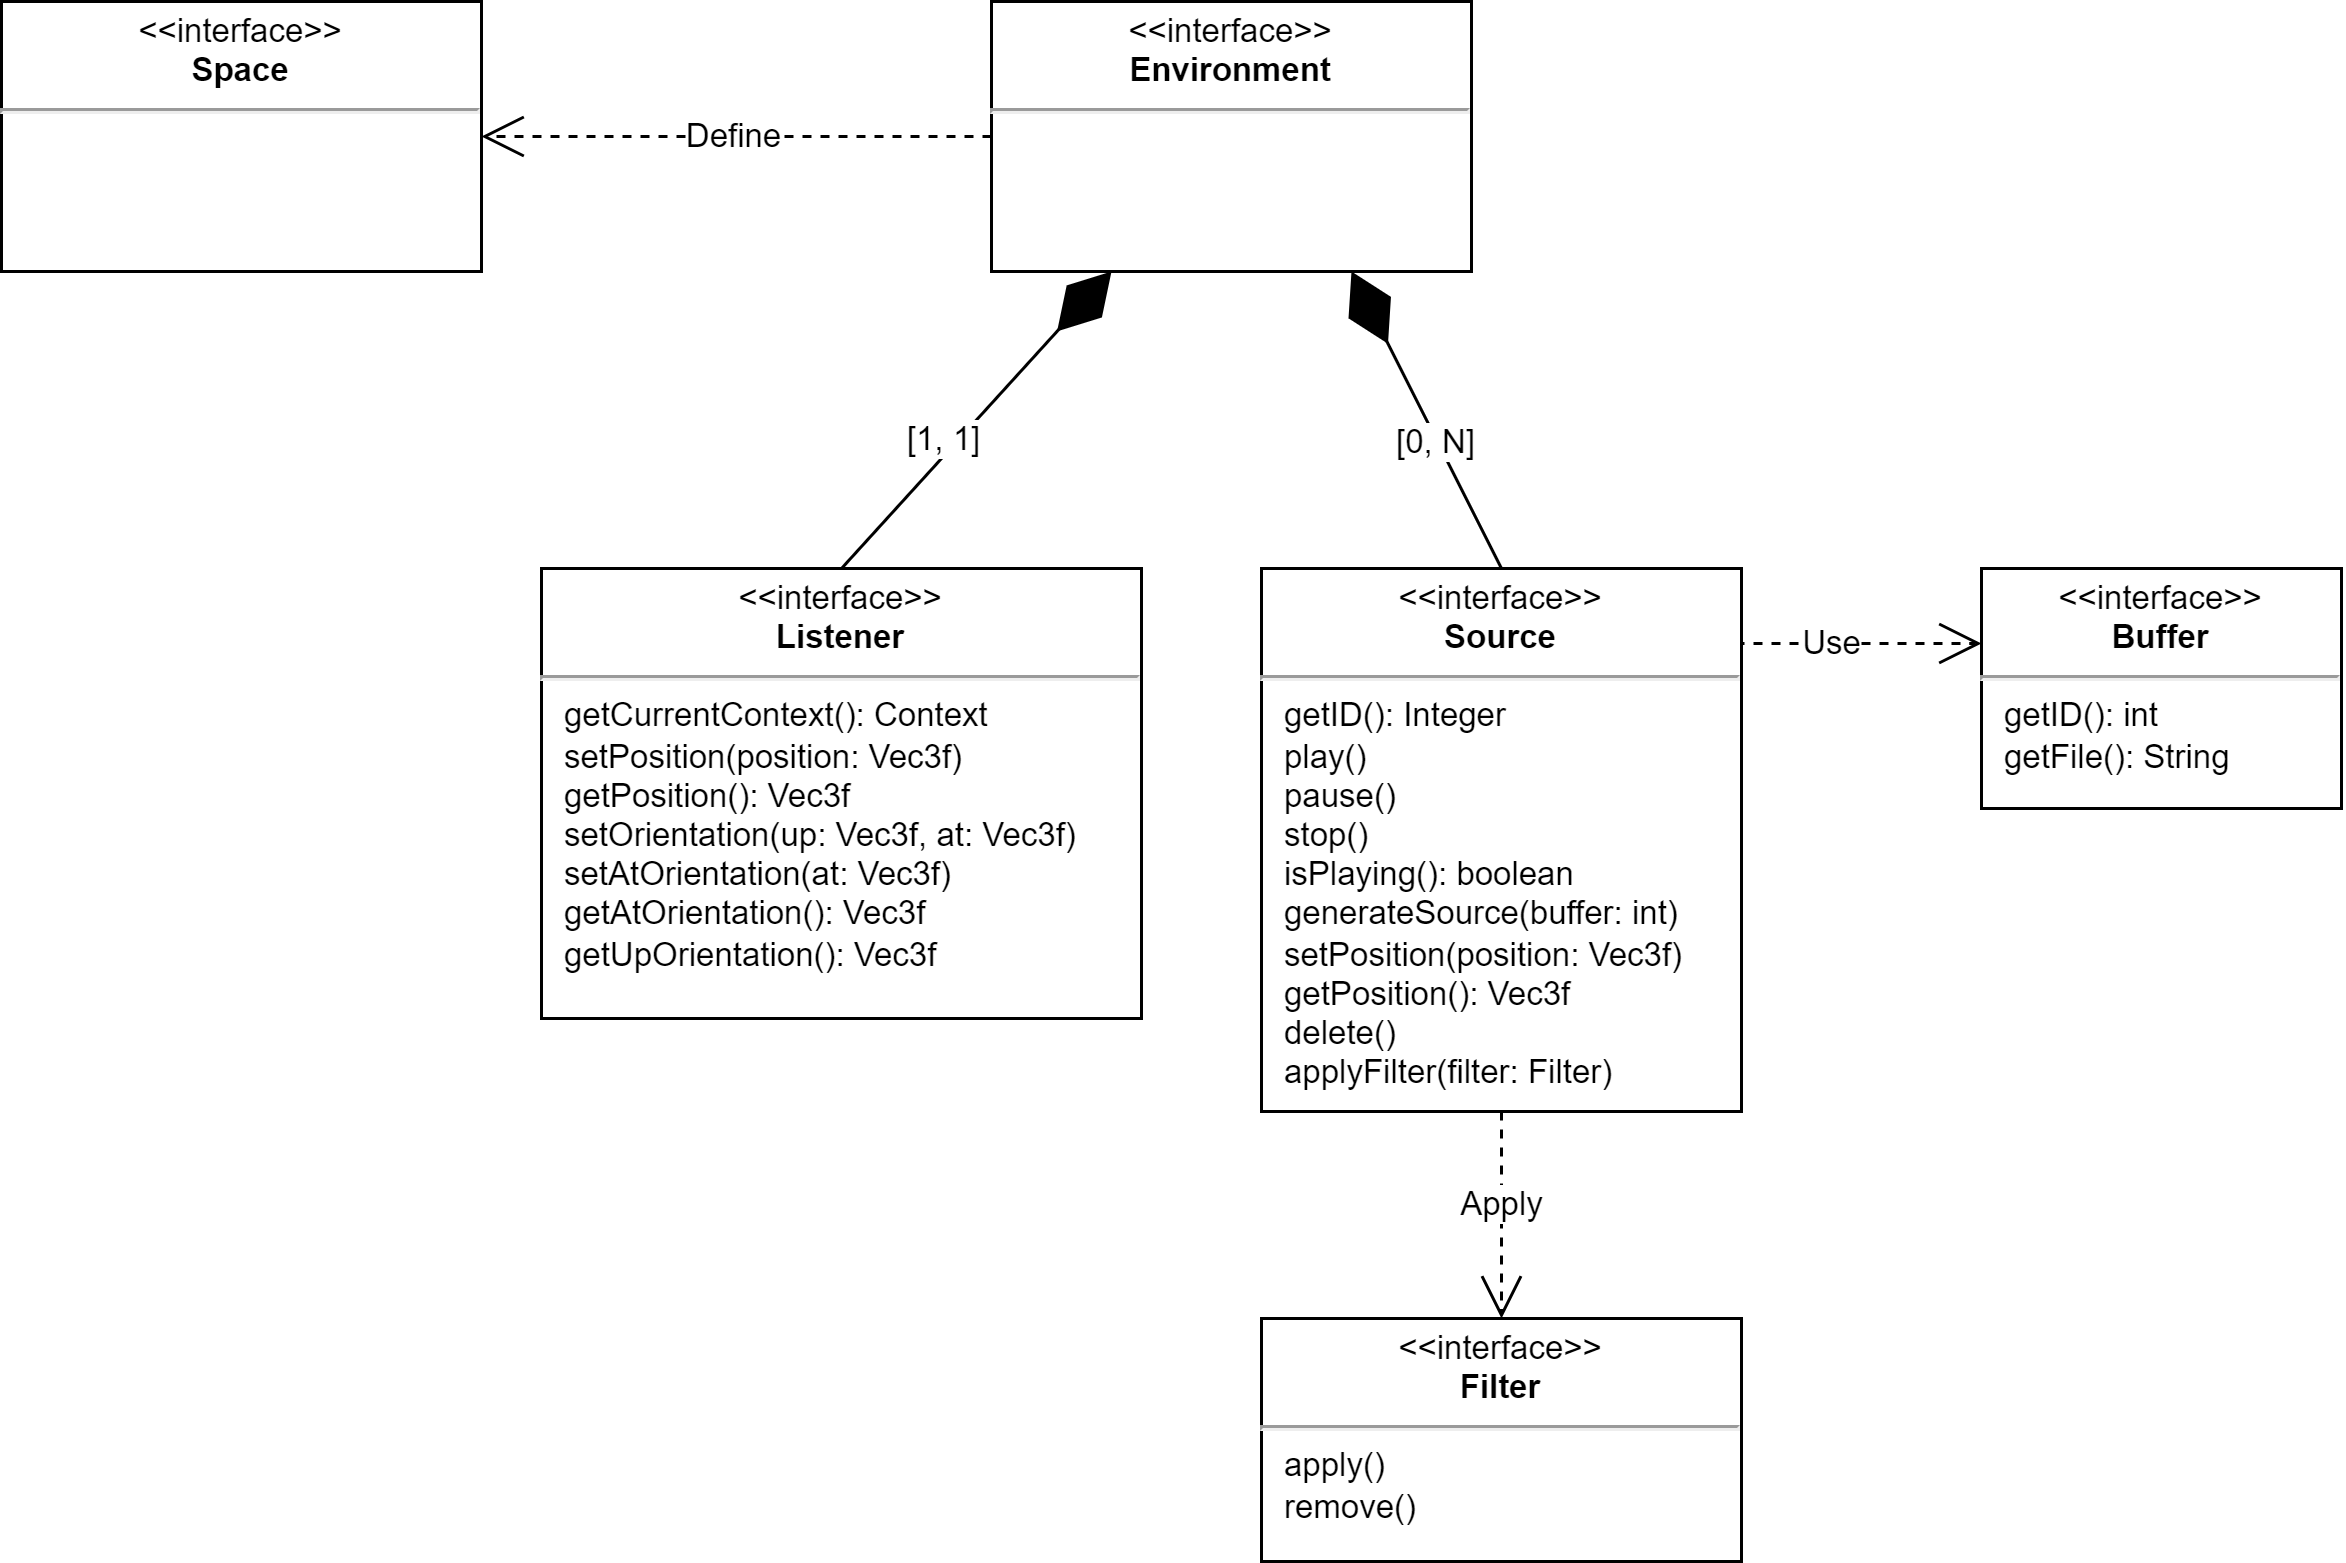
\includegraphics[width=\textwidth]{img/analysis.png}
\caption{Schema UML dell'analisi del problema, con rappresentate le entità principali ed i rapporti fra loro}
\label{img:analysis}
\end{figure}

\chapter{Design}
\section{Architettura}

\subsection*{MVC}
Nella strutturazione del progetto abbiamo cercato di seguire una linea standard con l'implementazione di MVC, cercando di rendere ogni parte di quest'ultimo il più modulare possibile dividendo in comparti ben definiti ogni sezione. Il model ha una struttura classica, invece abbiamo dovuto aggiungere componenti che avessero la funzione di coordinare controller e view.
%
\begin{figure}[H]
\centering{}
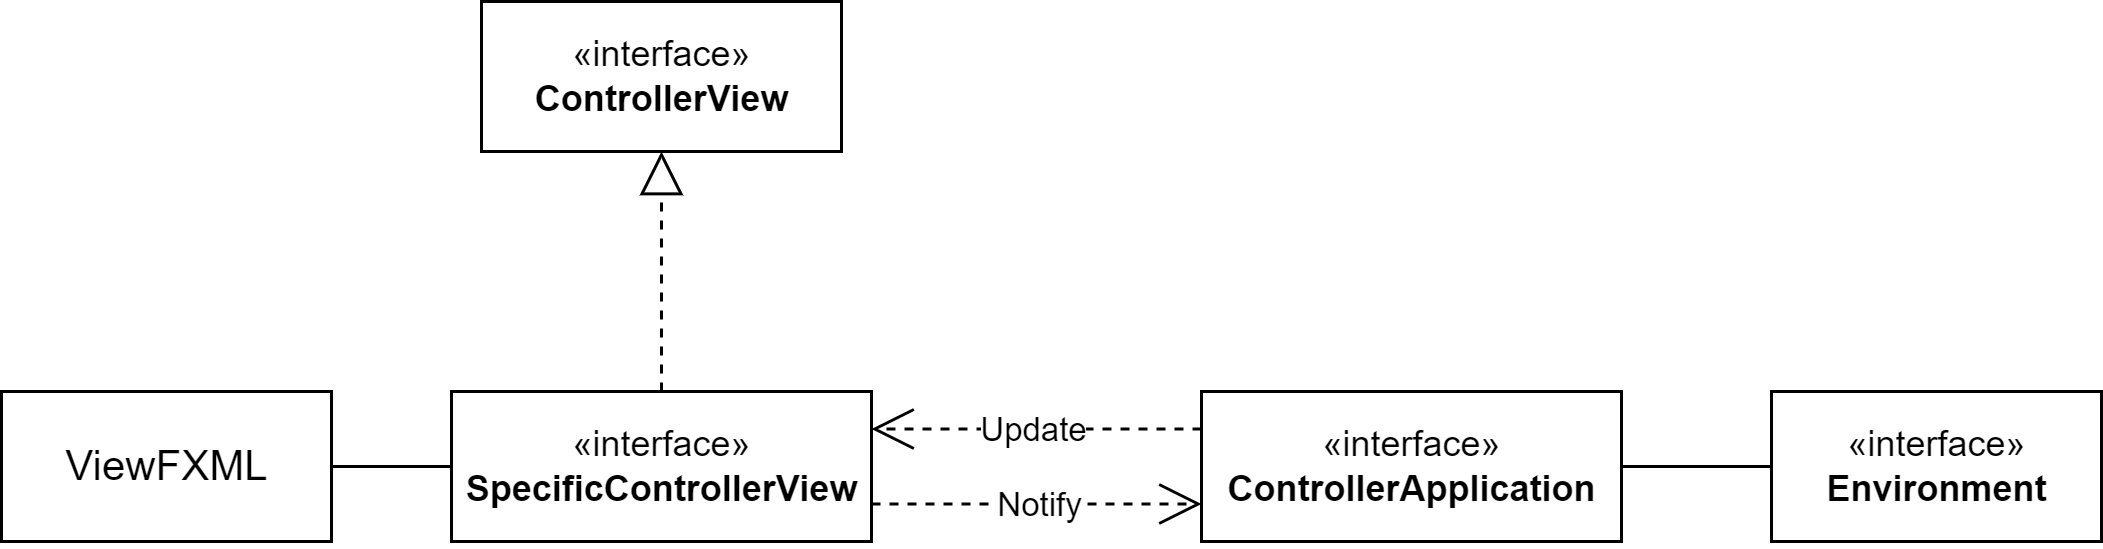
\includegraphics[width=\textwidth]{img/architecture/architecture.png}
\caption{Schema UML dell'MVC}
\label{img:analysis}
\end{figure}
%
\subsection*{Model}
L'interfaccia principale del model è offerta dall'Environment, che coordina le entità principali e ne contiene le istanze, ma ogni sua sottoparte ha comunque punti di ingresso per essere utilizzata dal proprio controller specifico, in modo da diversificare gli entry point e rendere il tutto più modulare.
%
\begin{figure}[H]
\centering{}
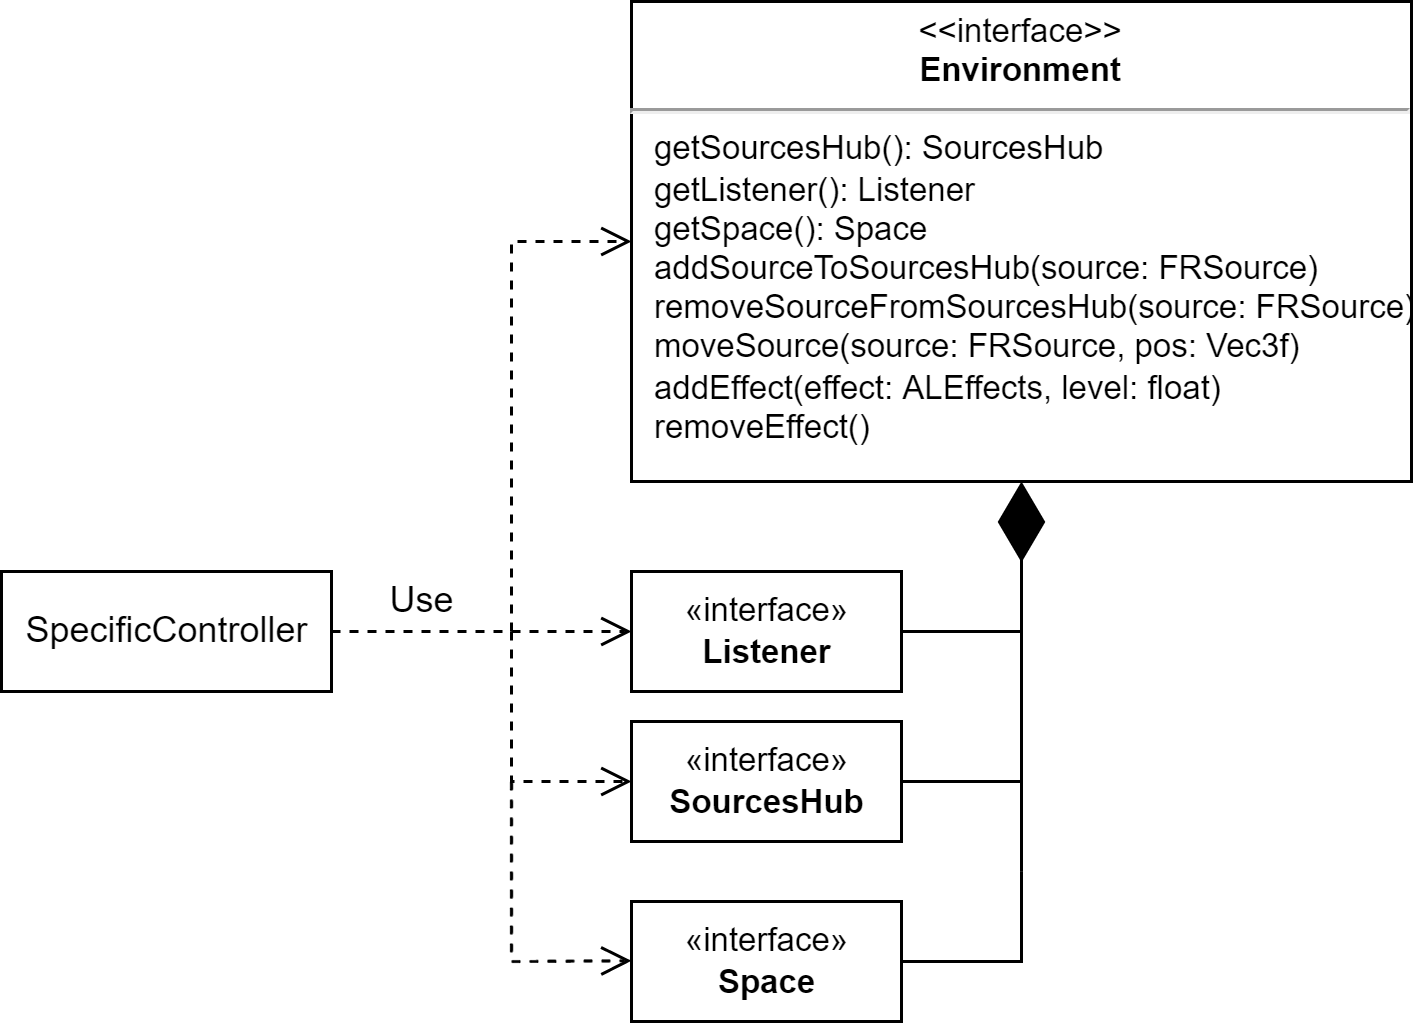
\includegraphics[width=\textwidth]{img/architecture/model.png}
\caption{Schema UML del model}
\label{img:analysis}
\end{figure}
%
\subsection*{Controller}
Abbiamo deciso di creare un MainController che gestisce tutti gli SpecificController in modo da rendere l'interazione tra essi più semplice. Esso mette a disposizione a ogni ControllerApplication la possibilità di accedere agli altri. 
\\La scelta di creare i vari SpecificController è dettata dal fatto che ognuno ha bisogno di gestire in modo specifico una parte di model e la creazione di un numero più ridotto di controller sarebbe stata troppo caotica e avrebbe limitato l'estendibilità e la manutenibilità del codice.
%
\begin{figure}[H]
\centering{}
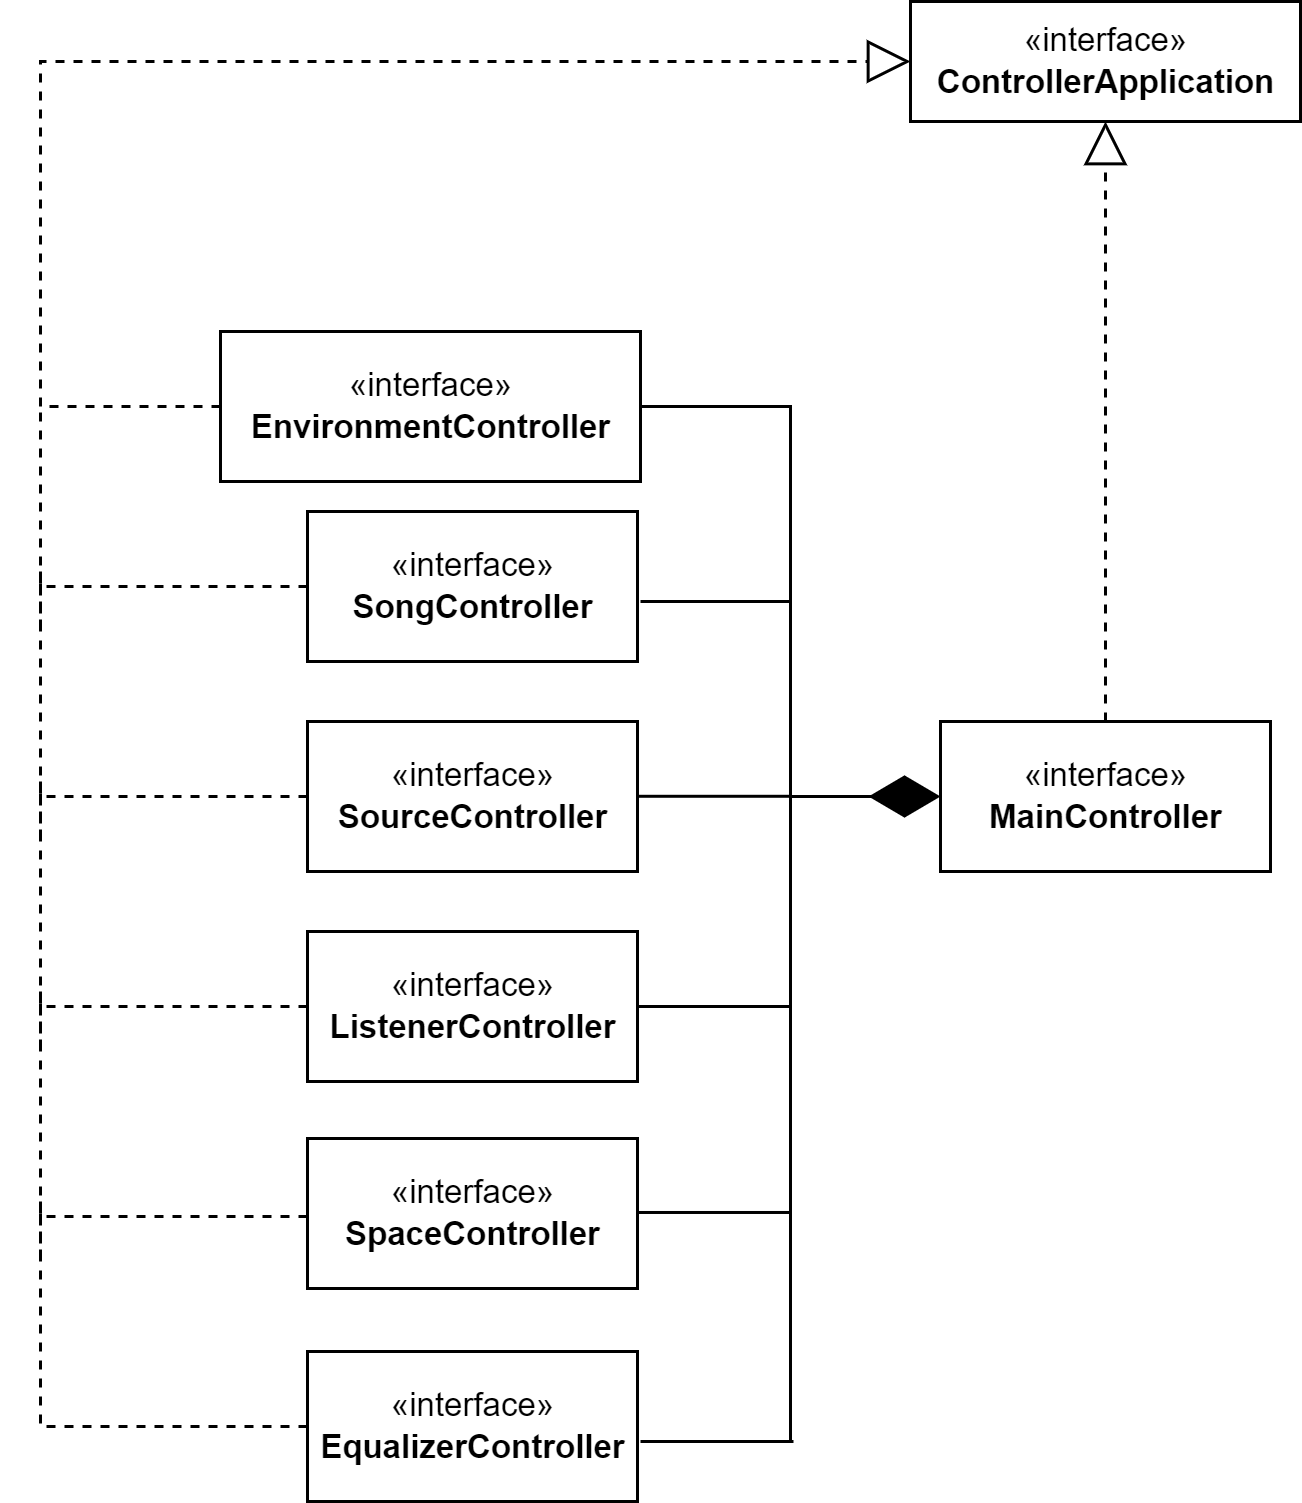
\includegraphics[width=\textwidth]{img/architecture/controller.png}
\caption{Schema UML dei controller}
\label{img:analysis}
\end{figure}
%
\subsection*{View}
Questa parte è risultata la più critica da progettare, data la poca esperienza con la tecnologia grafica utilizzata visto che abbiamo voluto mantenere una salda divisione tra le parti anche in questa fase di sviluppo. 
\\L'obiettivo era di traslare la modularità del model e del controller anche nella view e questo ci ha portato a definire diverse view per ogni entità principale. Abbiamo introdotto dei controller all'interno della parte di View relativa all'MVC, in modo da dividere la mera parte visiva da quella di controllo, permettendo ai ControllerView di gestire la specifica tecnologia grafica e creando delle interfacce view che non facessero trasparire la tecnologia utilizzata.

\begin{figure}[H]
\centering{}
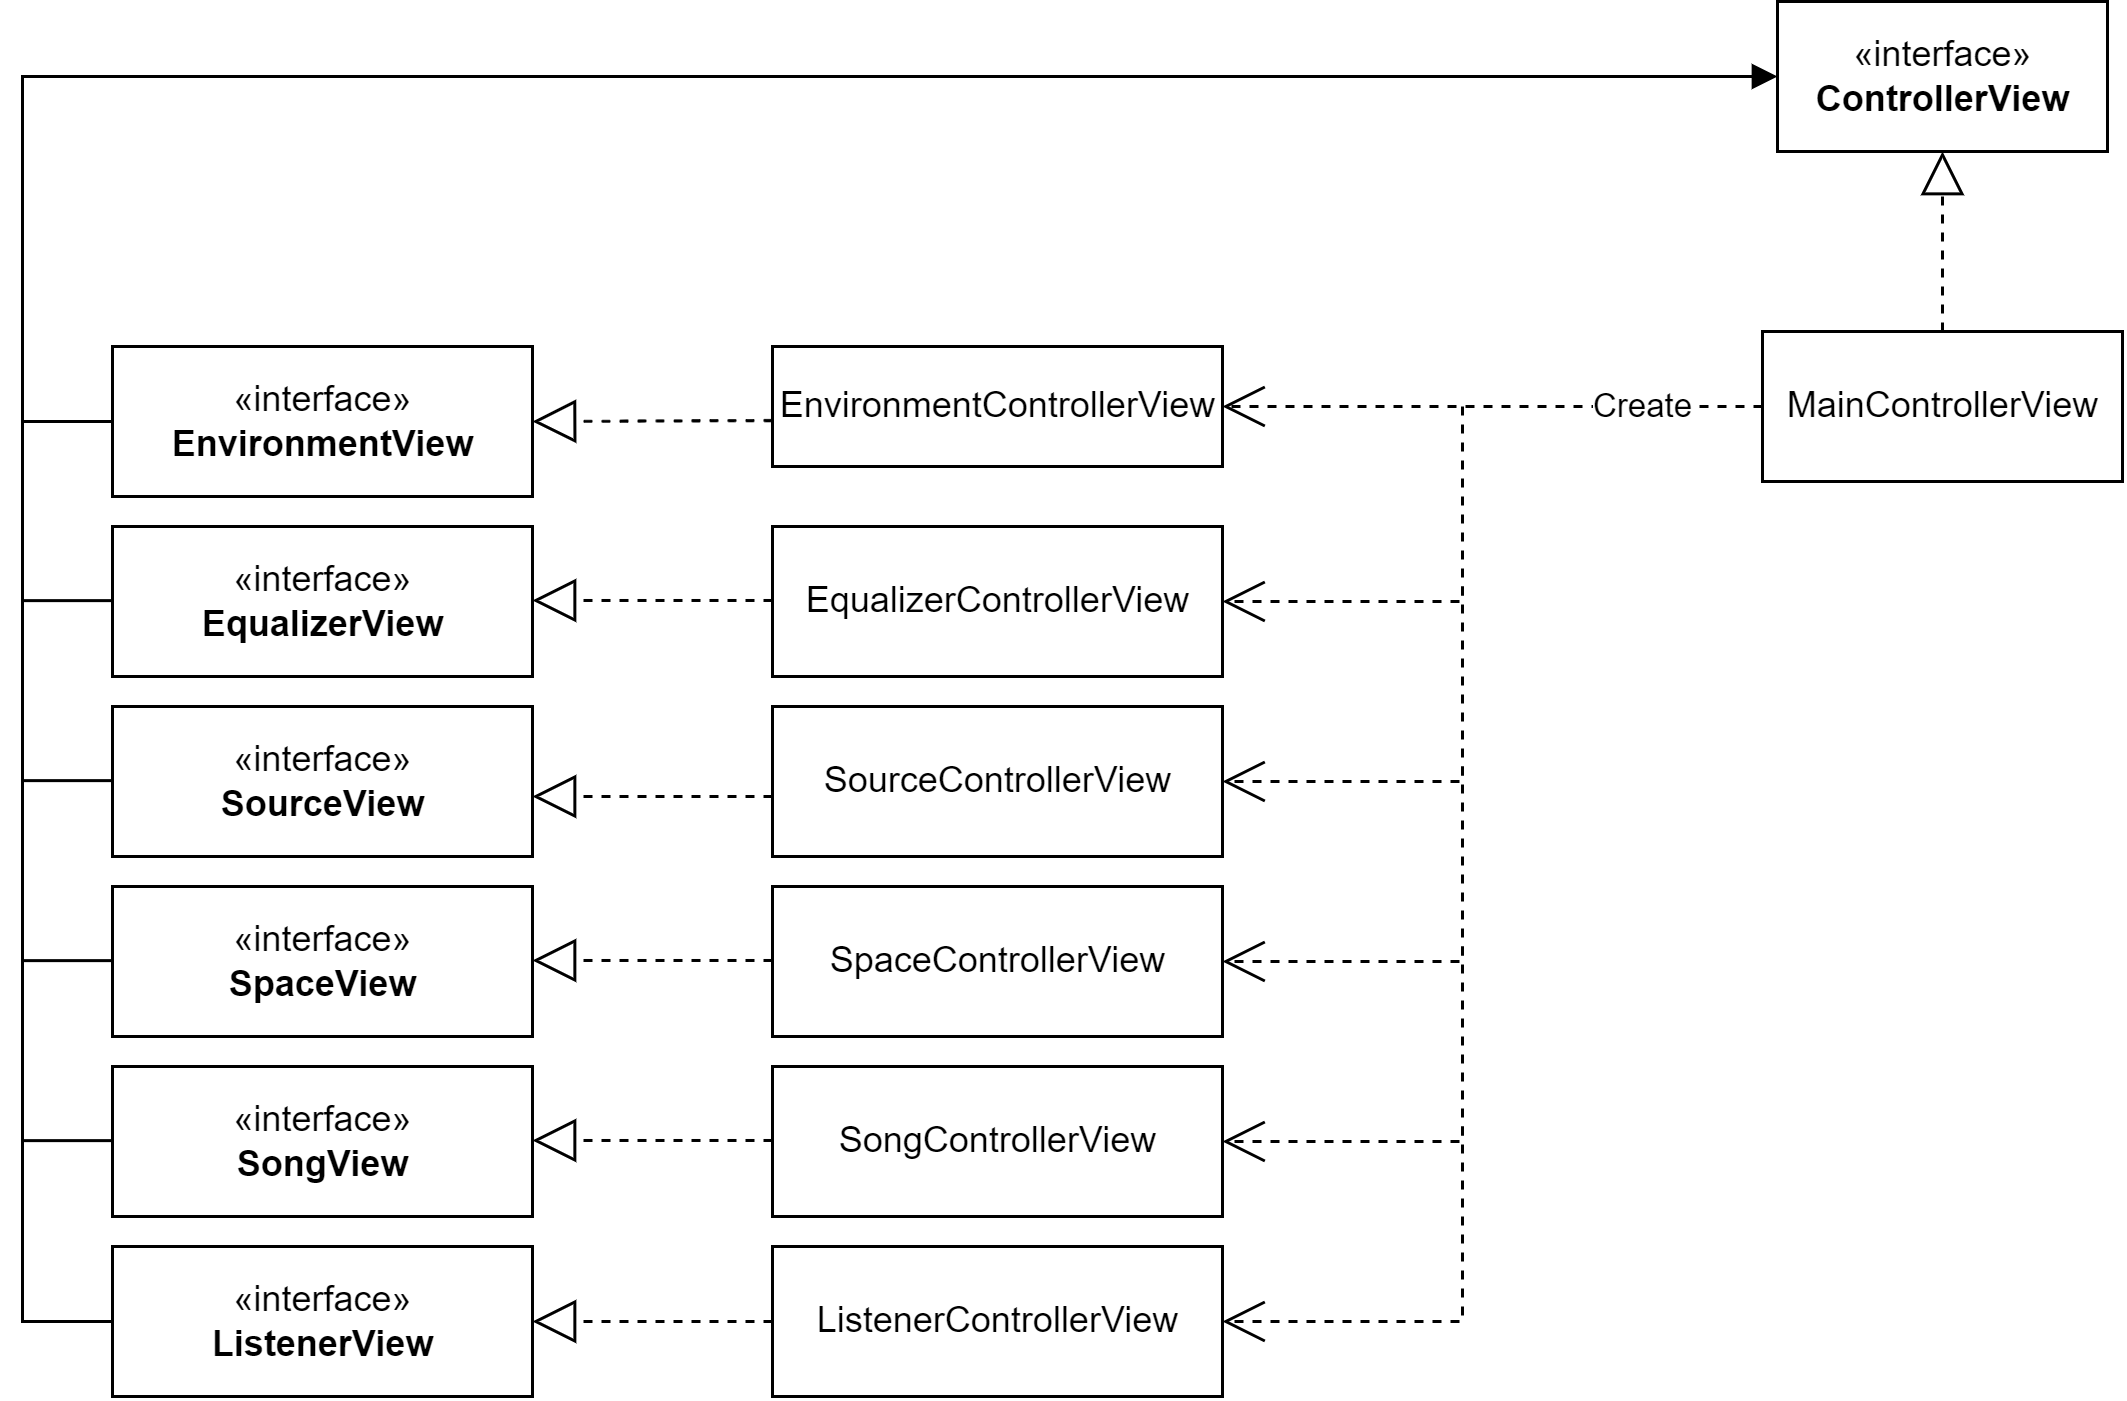
\includegraphics[width=\textwidth]{img/architecture/view.png}
\caption{Schema UML della view}
\label{img:analysis}
\end{figure}

\section{Design dettagliato}
\subsection*{Niccolò Mussoni}
Il mio dominio di lavoro è centrato su due argomenti:
\begin{itemize}
	\item I Buffer, che sulla base del file importato generano un ID univoco associato ad esso, attraverso il quale le sorgenti possono riprodurre il file. 
	\item Le estensioni, che riguardano la gestione di filtri ed effetti per le sorgenti.
\end{itemize}

\begin{figure}[H]
\centering{}
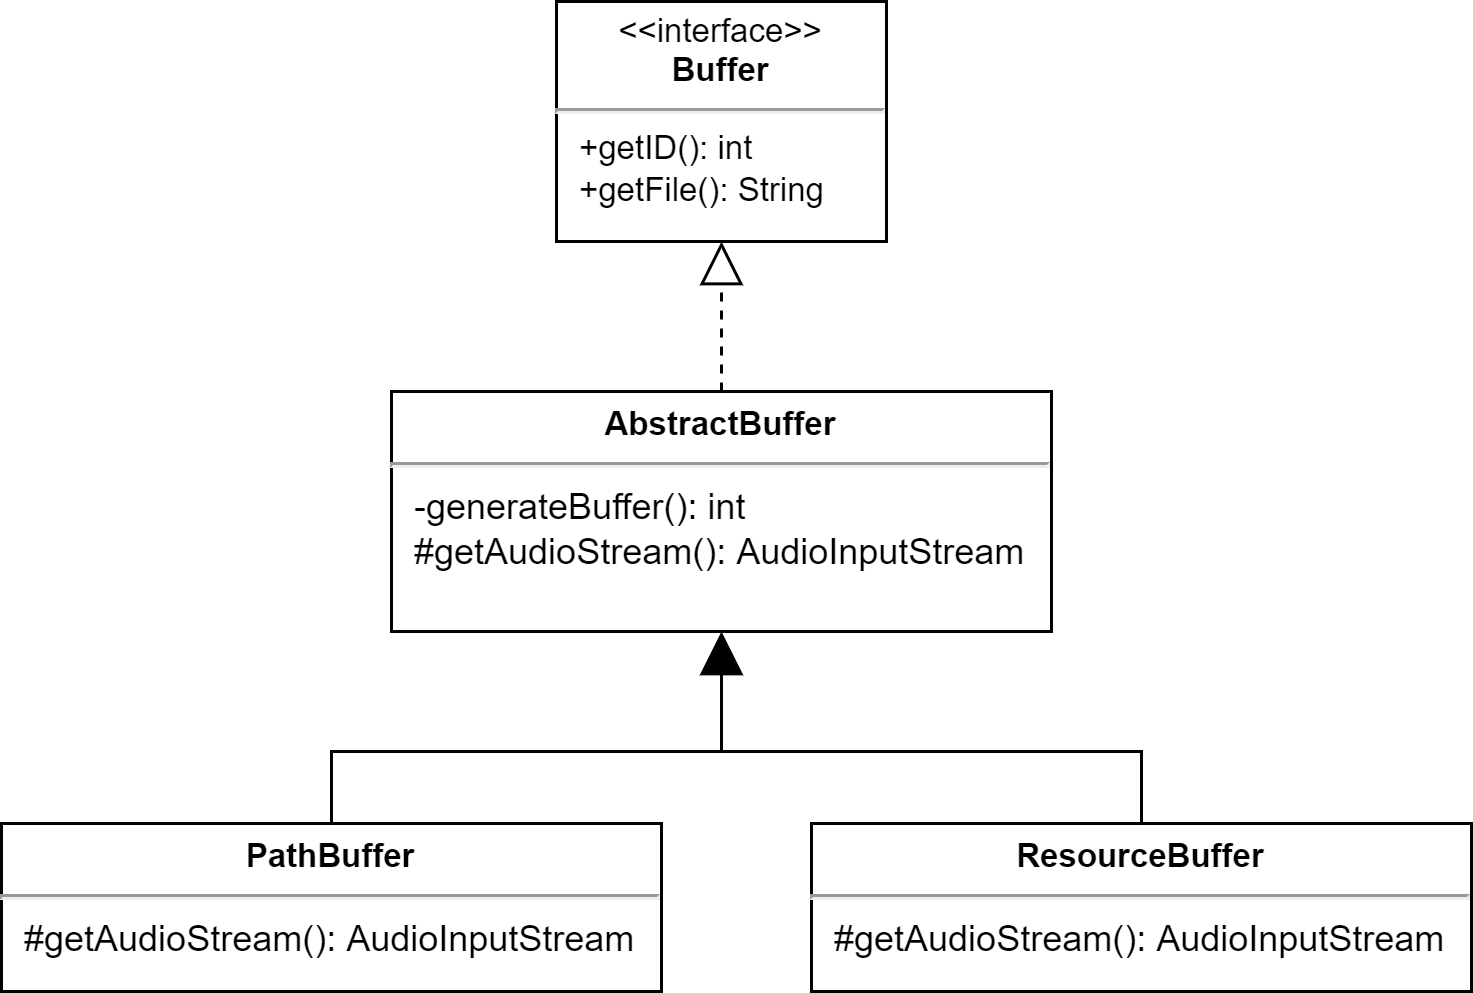
\includegraphics[width=\textwidth]{img/buffer/Buffer.png}
\caption{Rappresentazione UML dell’applicazione del pattern Template Method per i diversi tipi di Buffer}
\label{img:templatebuffer}
\end{figure}
Il primo problema da gestire è stato il fatto che il Buffer potesse essere generato sia da un file nel File System, sia da un file incluso nelle risorse del Classpath. Visto che i Buffer differiscono solo per come viene importato inizialmente lo Stream, per risolvere questo problema ho sfruttato il pattern template method, in modo da poter essere usato anche per altri tipi di Buffer non presenti nel progetto. Nel mio caso, il metodo template è generateBuffer, mentre il metodo primitivo è getAudioStream.
%
\begin{figure}[H]
\centering{}
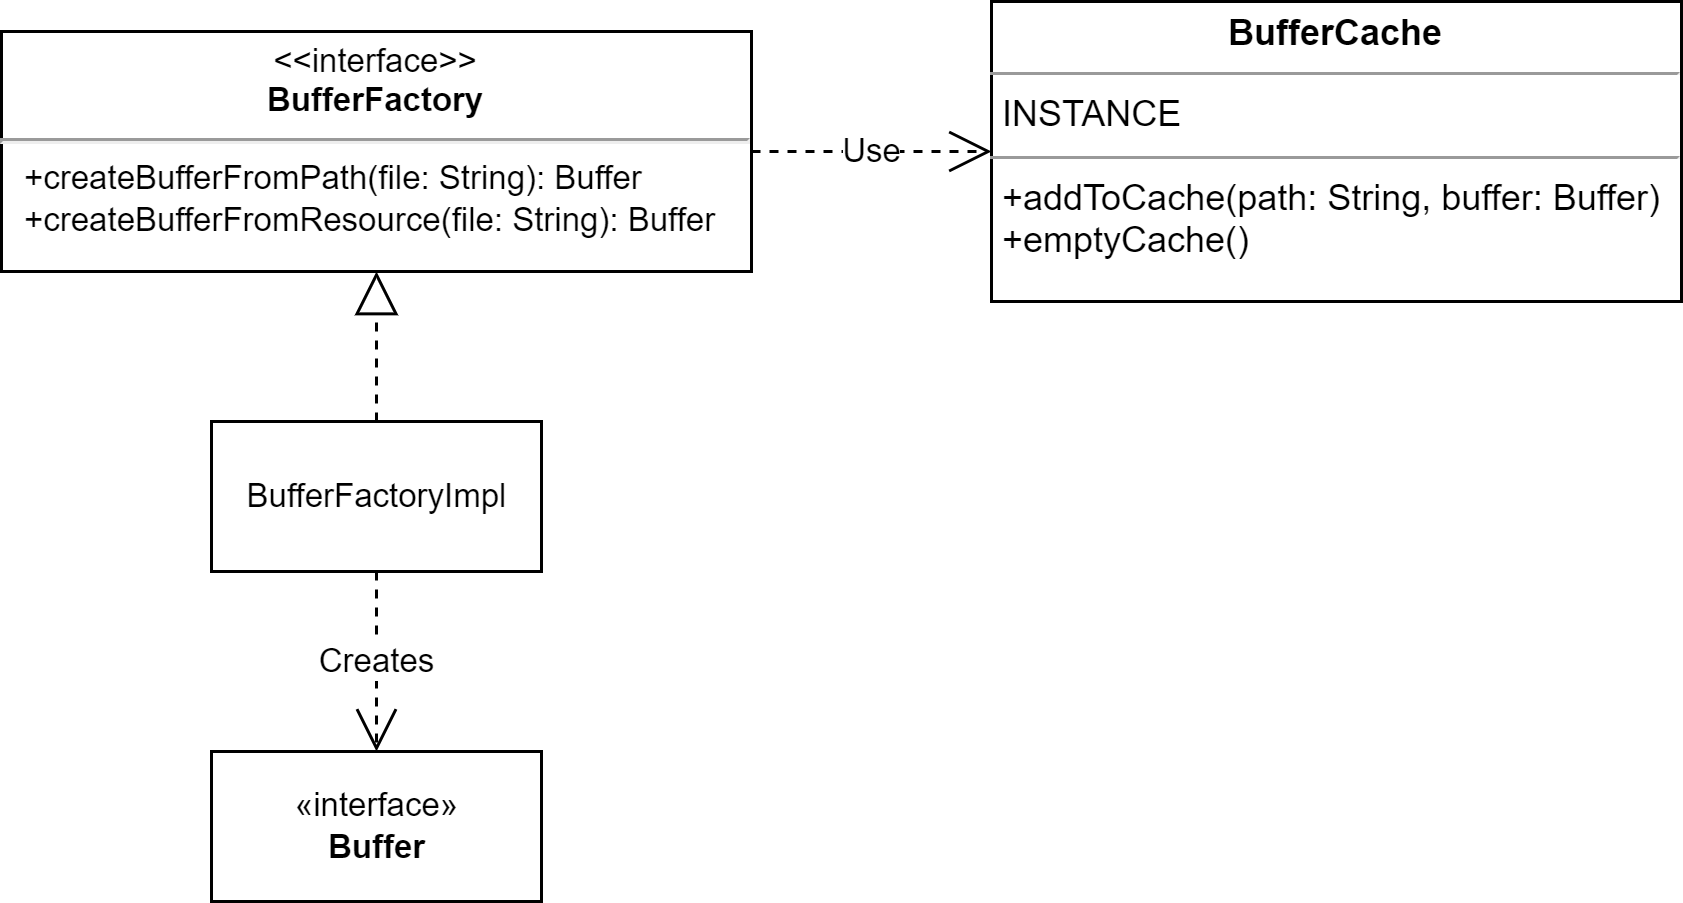
\includegraphics[width=\textwidth]{img/buffer/BufferImport.png}
\caption{Rappresentazione UML della Factory per Buffer e dell’applicazione del pattern Singleton per il caching}
\label{img:cachebuffer}
\end{figure}
Il secondo problema da gestire era evitare Buffer duplicati e per risolvere ciò mi sono affidato a un istanza Singleton che potesse fare da cache in maniera thread-safe, grazie alla versione di J. Bloch. La factory, prima di creare un nuovo Buffer, controlla che non sia già presente nella cache e successivamente procede a crearne uno nuovo.
%
\begin{figure}[H]
\centering{}
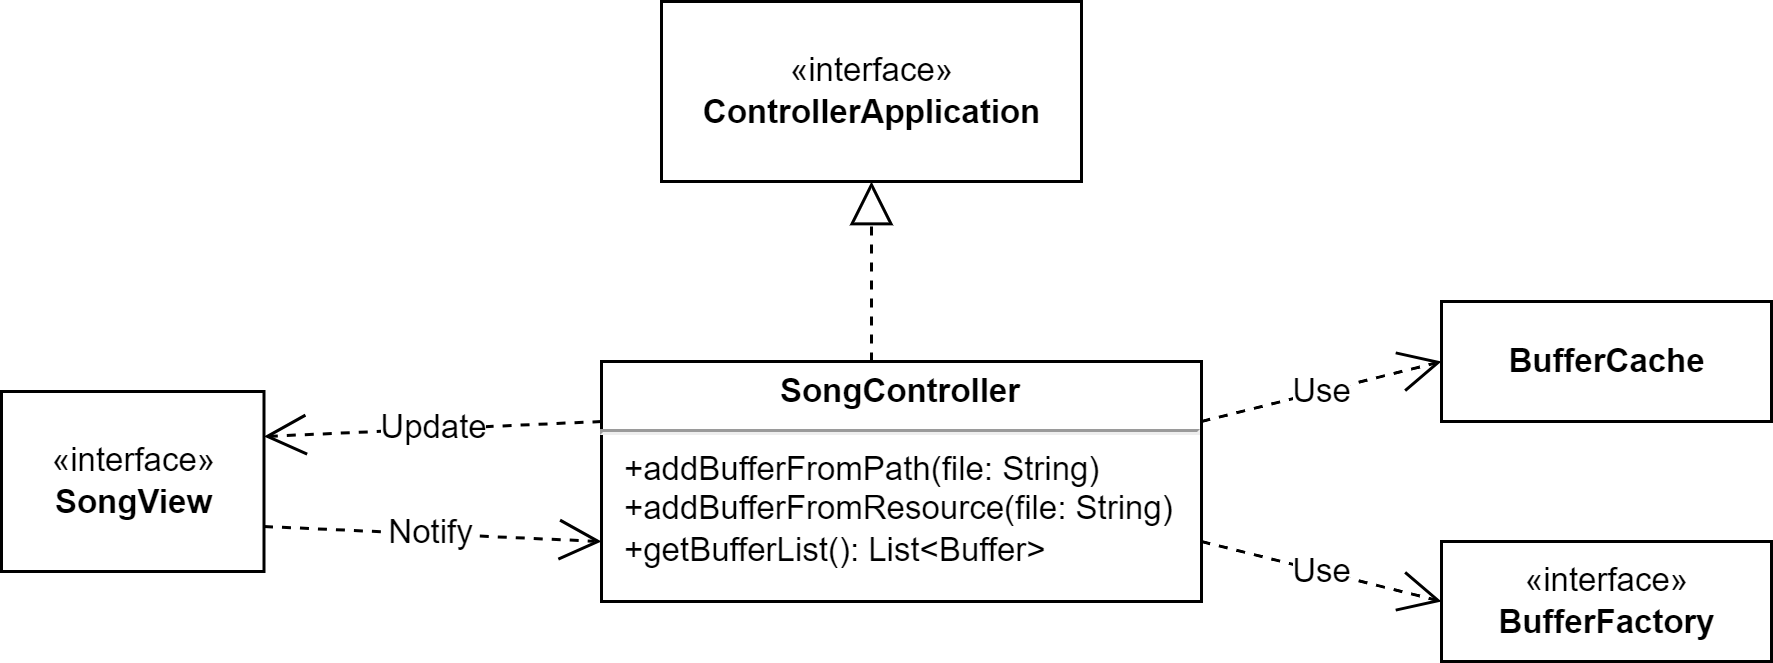
\includegraphics[width=\textwidth]{img/buffer/BufferMVC.png}
\caption{Rappresentazione UML della Factory per Buffer e dell’applicazione del pattern Singleton per il caching}
\label{img:buffermvc}
\end{figure}
Quando dalla view viene richiesta l’importazione di un file, esso viene trattato come PathBuffer, in quanto viene selezionato dall’utente. Al momento dell’inizializzazione invece tutti i file audio presenti come risorse del progetto vengono trattati come ResourcePath. Questo mi ha aiutato a poter differenziare anche i metodi nel controller senza ricorrere a variabili booleane o intere per identificare che tipo di file fosse. Il controller, dopo aver ricevuto la richiesta di creare un nuovo buffer, chiama la factory, che procede a creare il Buffer, che se non è presente viene aggiunto anche nella cache. Inoltre la cache è risultata utile anche per poter aggiornare la view successivamente al caricamento di un file, in quanto il controller ricava il nome dei file presenti nella cache e notifica alla view di aggiornarsi sulla base della lista dei file.
%
\begin{figure}[H]
\centering{}
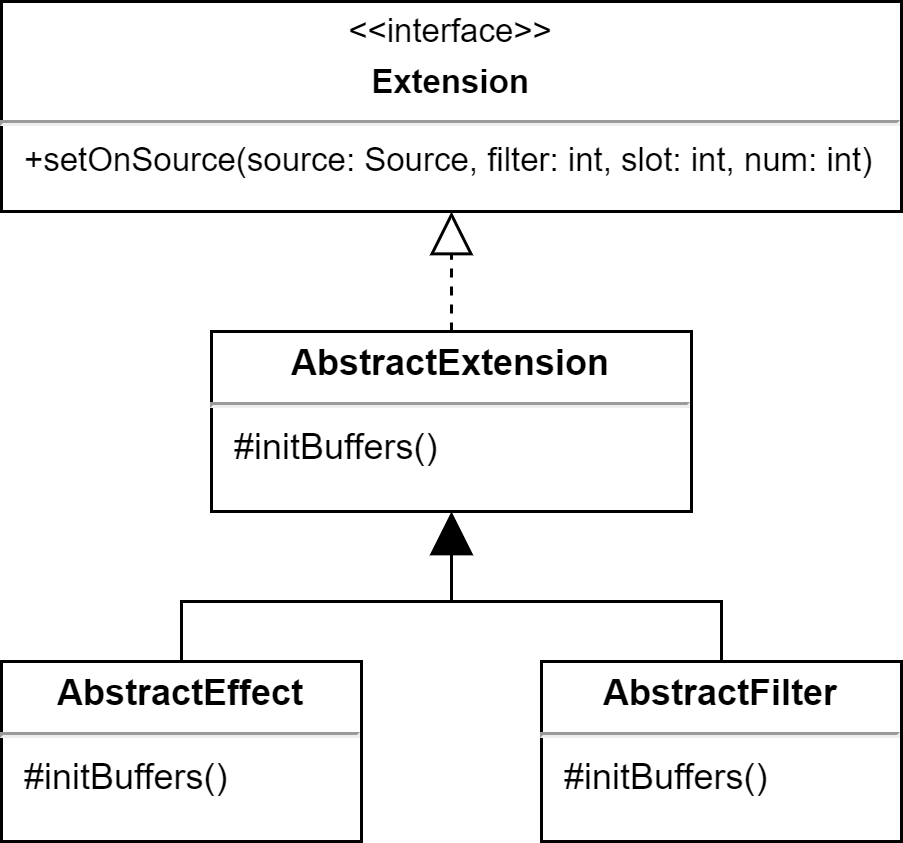
\includegraphics[width=\textwidth]{img/extension/Extensions.png}
\caption{Rappresentazione UML della parte comune delle estensioni}
\label{img:extensions}
\end{figure}
Sia filtri che effetti condividono la parte in cui vengono applicati alla sorgente, ma non i buffer necessari alla creazione di essi, quindi ho deciso di creare un’interfaccia comune per la parte di applicazione, e successivamente una sua implementazione astratta, che implementa l’applicazione delle estensioni, ma non l’inizializzazione, la quale viene lasciata alle due classi che ereditano. Invece la creazione/rimozione del filtro o effetto attraverso la libreria era differente, quindi ho sfruttato due interfacce separate, mostrate nelle due figure successive.
%
\begin{figure}[H]
\centering{}
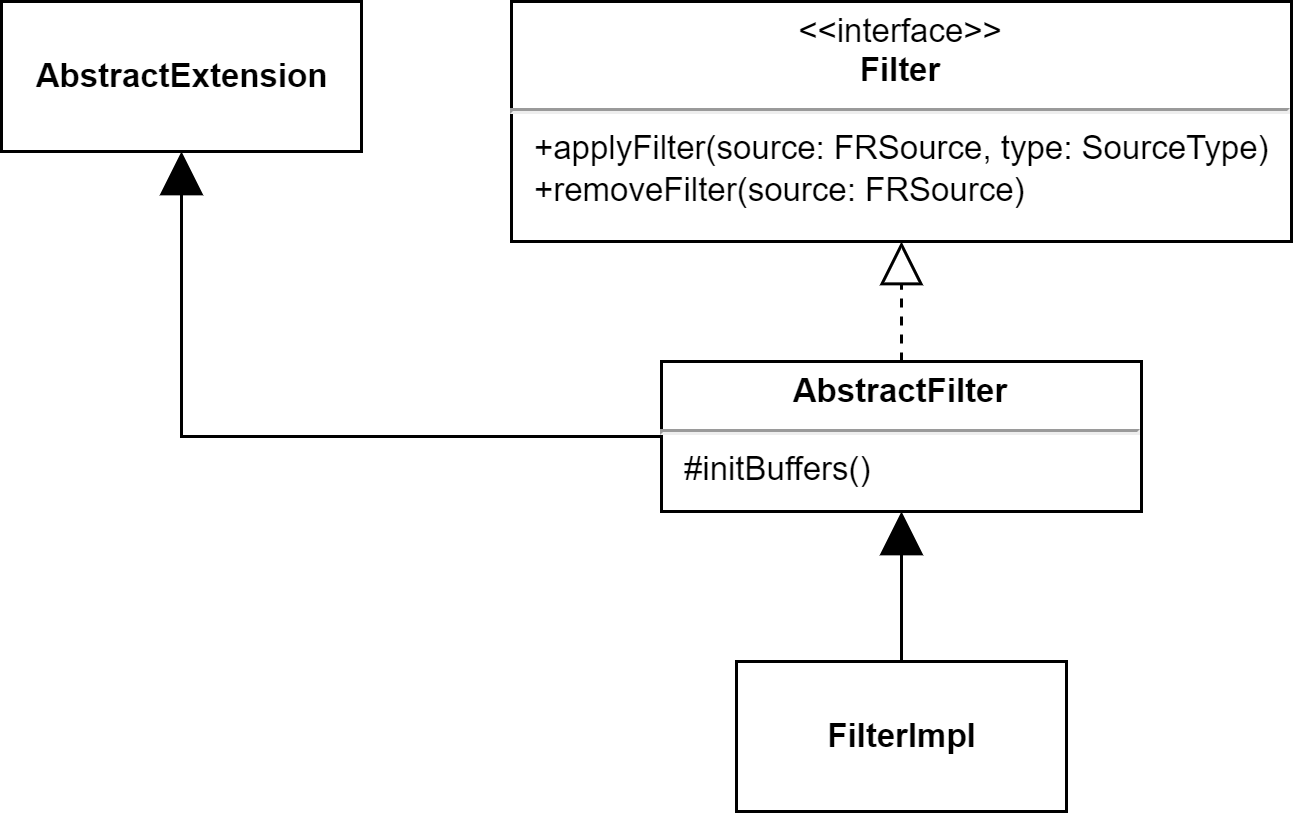
\includegraphics[width=\textwidth]{img/extension/Filter.png}
\caption{Rappresentazione UML della gestione dei filtri}
\label{img:filter}
\end{figure}
I filtri hanno un valore impostato a priori per i tre tipi di filtro (passa-basso, passa-banda, passa-alto), quindi mi è bastato solo implementare la creazione e la rimozione. 
%
\begin{figure}[H]
\centering{}
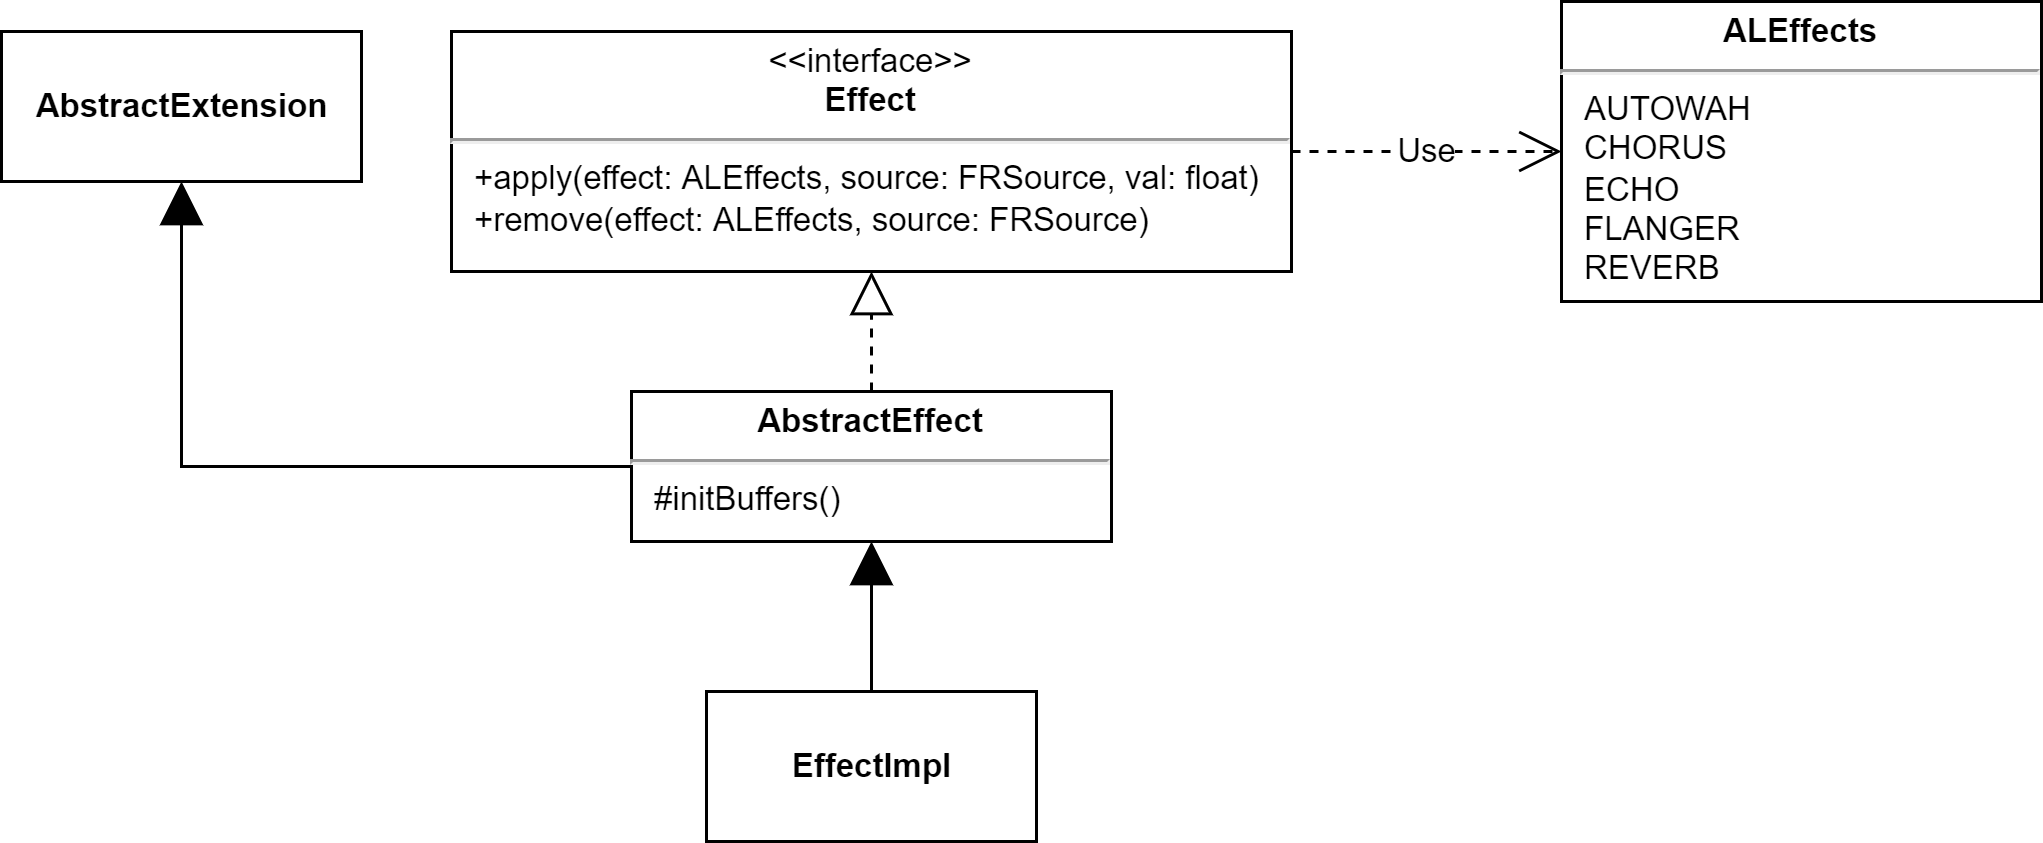
\includegraphics[width=\textwidth]{img/extension/Effect.png}
\caption{Rappresentazione UML della gestione degli effetti attraverso enum}
\label{img:effects}
\end{figure}
Per la gestione degli effetti e dei suoi attributi mi sono affidato ad un enum con costruttore, che mi permettesse in maniera veloce di cambiare i parametri di un dato effetto, come valore massimo e minimo, e di aggiungerli o rimuoverli. A differenza dei filtri, il valore degli effetti dipende dall’interazione dell’utente con la view.
%
\begin{figure}[H]
\centering{}
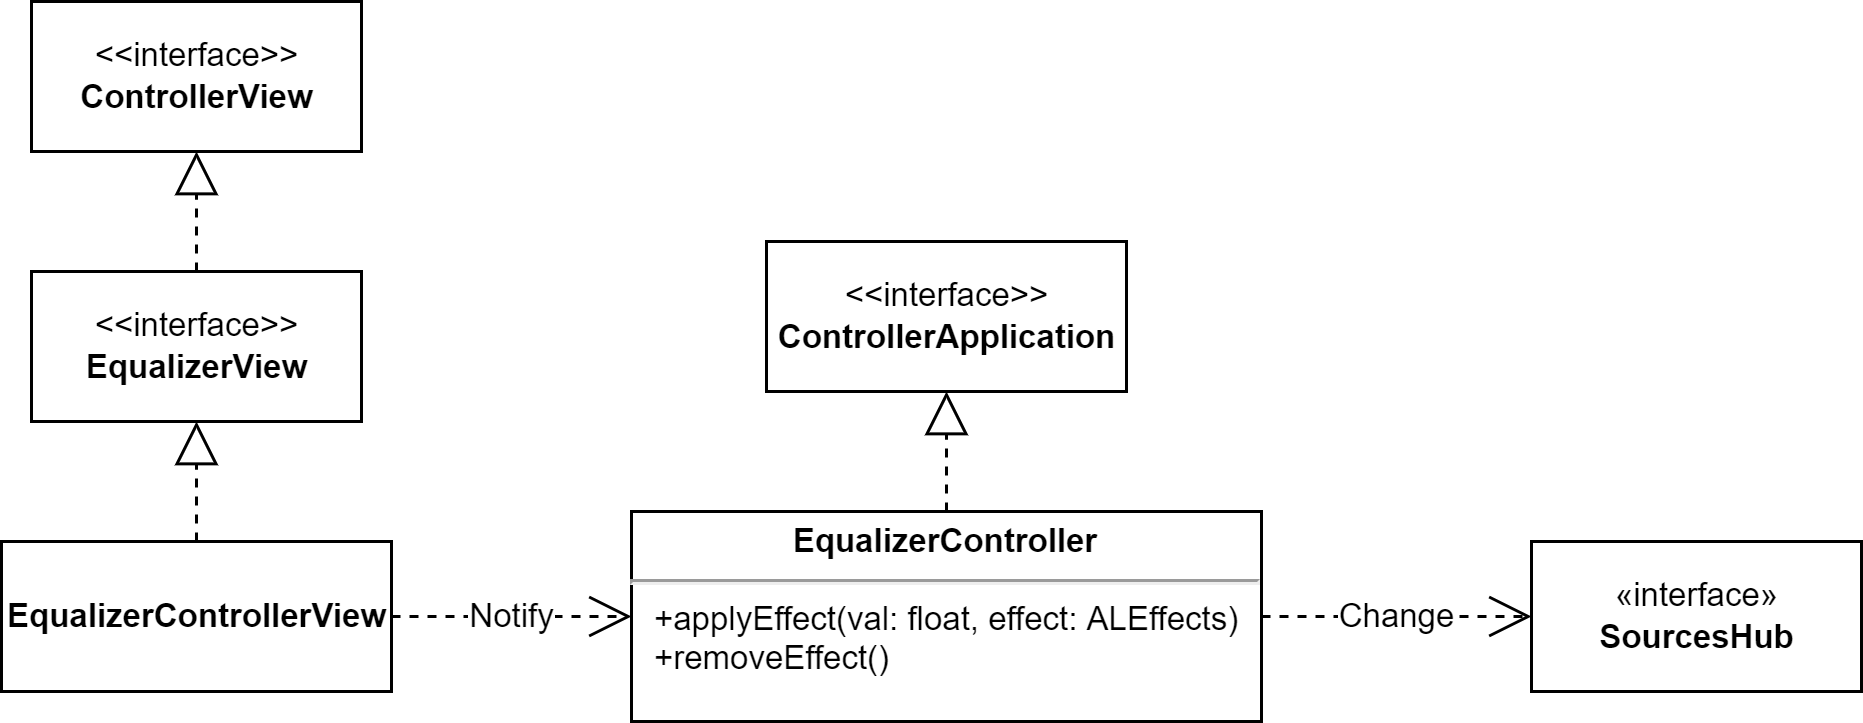
\includegraphics[width=\textwidth]{img/extension/EffectsMVC.png}
\caption{Rappresentazione UML dello schema MVC relativo all’utilizzo degli effetti}
\label{img:effectsmvc}
\end{figure}
L’interazione dell’utente con l’equalizzatore, composto da slider, mi ha permesso di ricavare il valore dell’effetto il quale viene passato al controller che notificherà a tutte le sorgenti di applicare il determinato effetto con il determinato valore. In questa parte di MVC il controller non notifica nulla alla view, in quanto si tratta di un equalizzatore che non ha bisogno di aggiornare l’interfaccia in base alle azioni dell’utente.
%
\subsection*{Alessandro Sciarrillo}
Il dominio su cui ho lavorato è quello delle sorgenti che comprende la loro implementazione sia come singole ma anche come gruppo.

Inizialmente mi sono occupato della strutturazione delle sorgenti che modellano i diversi tipi di speakers nelle sezioni a loro comuni e non. Per agevolare la riusabilità ho optato per una classe più primitiva "Source" che riguardasse l'utilizzo di base comune a ogni speaker, lasciando a "FRSource"(Frequency Range Source) solamente le funzioni relative al range di frequenze:
%
\begin{figure}[H]
\centering{}
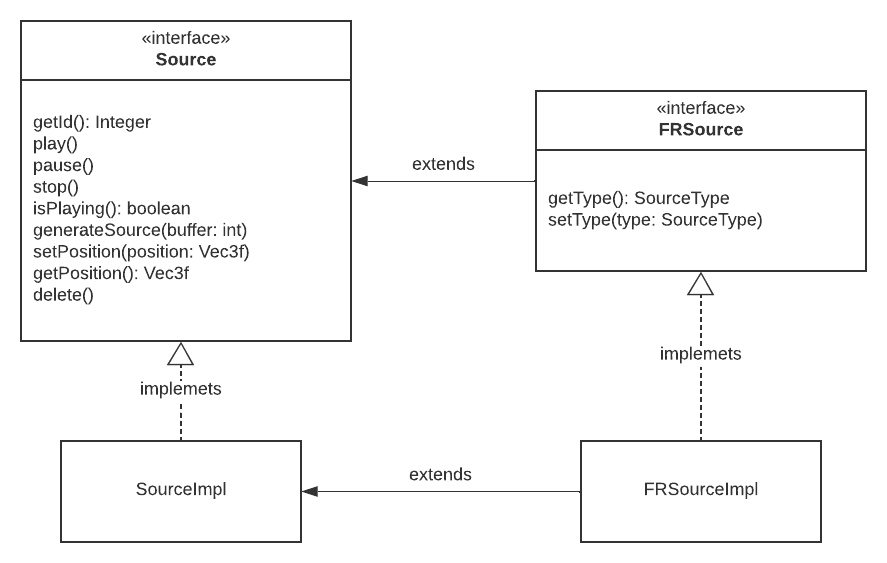
\includegraphics[width=\textwidth]{img/source/Source-FRSource.png}
\caption{Riuso del codice da parte di FRSource.}
\label{img:sourcesHub}
\end{figure}

Così facendo il codice scritto per la versione base "Source" è stato riusato come fondamenta della versione più avanzata "FRSource"
lasciando però libertà in implementazioni future di creare altre forme avanzate di Source che non necessariamente debbano gestire
range di frequenze.

Uno dei principali aspetti del mio lavoro riguarda inoltre l'implementazione di speaker con range di frequenza differenti, qui ho incontrato uno dei problemi strutturali maggiori, le qualità che volevo imprimere nella soluzione erano:
\begin{itemize}
	\item Le sorgenti con range di frequenza eterogenei dovevano essere riconducibili a una classe padre comune a tutte.
	\item La quantità di codice necessaria ad implementare i vari tipi di range doveva essere estremamente ridotta.
\end{itemize}
Quindi la prima soluzione a cui ho pensato aveva questa forma:
%
\begin{figure}[H]
\centering{}
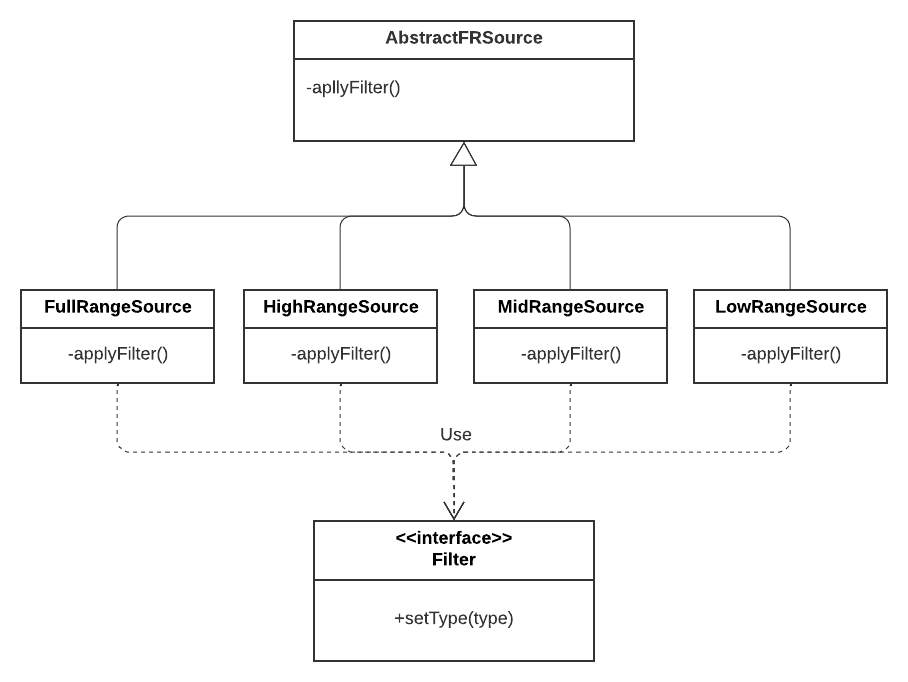
\includegraphics[width=\textwidth]{img/source/FRSource(ereditarieta).png}
\caption{Prima "bozza" rappresentazione schematica FRSource.}
\label{img:sourcesHub}
\end{figure}

Inizialmente sembrava scontata la necissità di un Template method per il metodo applyFilter, ma dopo una analisi più dettagliata del tipo di operazioni e lo scopo 
fondamentale di questa entità, cioè il poter cambiare in modo molto dinamico il range di frequenza sono arrivato alla conclusione che un implementazione del template method avrebbe appesantito il codice dell'utilizzatore in quanto il cambiamento di range di frequenza per una istanza (ad esempio da High a Low) avrebbe comportato la creazione di una nuova istanza della classe relativa alla nuova frequenza che sarebbe andata a sostituire quella precedente. In sostanza un cambiamento di frequenza avrebbe comportato il passaggio della source da una classe ad un altra quando la differenza tra quest'ultime è unicamente l'implementazione del metodo con cui impostare il proprio range di frequenza al buffer a loro associato.
Così ho optato per la costruzione di una classe FRSource che avesse un proprio tipo di range di frequenza SourceType:
%
\begin{figure}[H]
\centering{}
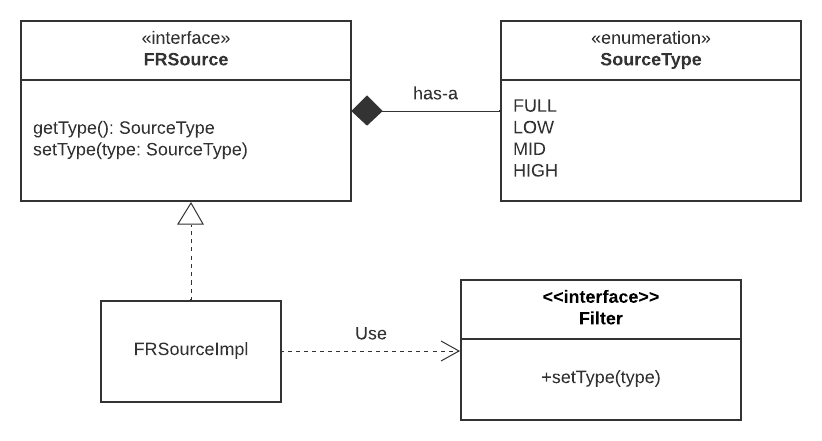
\includegraphics[width=\textwidth]{img/source/SourceType.png}
\caption{Rappresentazione struttura FRSource con ralazione "has-a" relativa a SourceType e l'implementazione FRSourceImpl che usa Filter.}
\label{img:sourcesHub}
\end{figure}

In conclusione con questa struttura cambiare range di frequenza a uno speaker comporta unicamente una chiamata al metodo setType. Con altre strutture valutate invece sorgeva sempre la necessità di compiere operazioni aggiuntive dal chiamante che doveva effettuare il cambio di range.

In seguito primo passo nella gestione di un insieme di speaker invece è stato quello di ideare una struttura che permettesse di gestire le sorgenti come singole ma anche come un gruppo e da qui è nato il concetto di SourcesHub:
%
\begin{figure}[H]
\centering{}
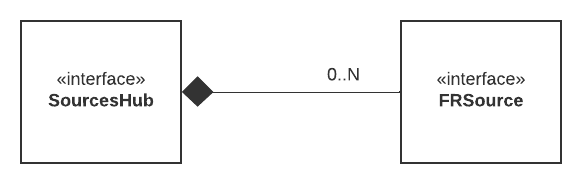
\includegraphics[width=\textwidth]{img/source/SourcesHub-Source.png}
\caption{Rappresentazione schematica composizione di SourcesHub.}
\label{img:sourcesHub}
\end{figure}

SourcesHub è come spiega il nome è un Hub che permette di avere un insieme di Sources al suo interno e la sua funzione è indubbiamente utile per un progetto di questo tipo che spesso necessita di eseguire operazioni o procedure uguali su più di una Source che fa parte dello stesso contesto.
%
\begin{figure}[H]
\centering{}
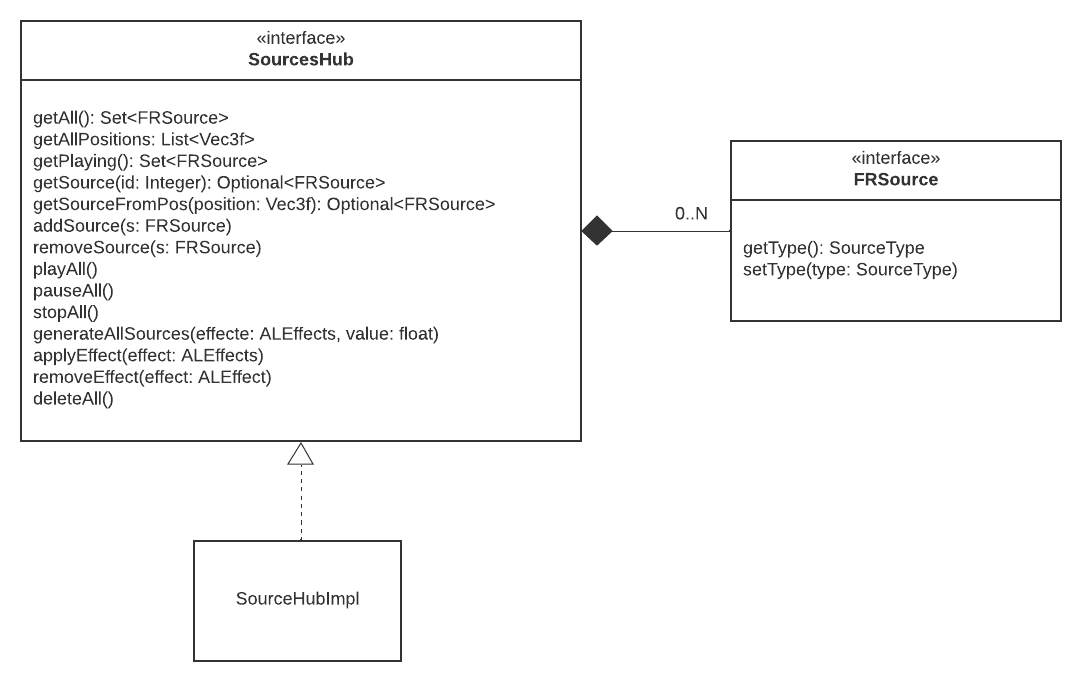
\includegraphics[width=\textwidth]{img/source/SourcesHub-Source-deeper.png}
\caption{Rappresentazione schematica composizione di SourcesHub.}
\label{img:sourcesHub}
\end{figure}

La gestione dell'MVC è alquanto semplice, il SourceController ha una comunicazione bilaterale con SourceControllerView, questo perchè la View deve richiedere operazioni in risposta alle interazione con l'utente (aggiunta, rimozione e modifica di uno speaker) e allo stesso tempo il Controller deve poter aggiornare la View quando lo speaker selezionato cambia e le componenti della view devono essere aggiornate per essere mantenute consonsistenti alle informazioni dello speaker correntemente selezionato.
Il controller inoltre effettua i cambiamenti sulle sorgenti che sono contenute in SourcesHub all'interno di Environment interfacciandosi a lato pratico con EnvironmentController.
%
\begin{figure}[H]
\centering{}
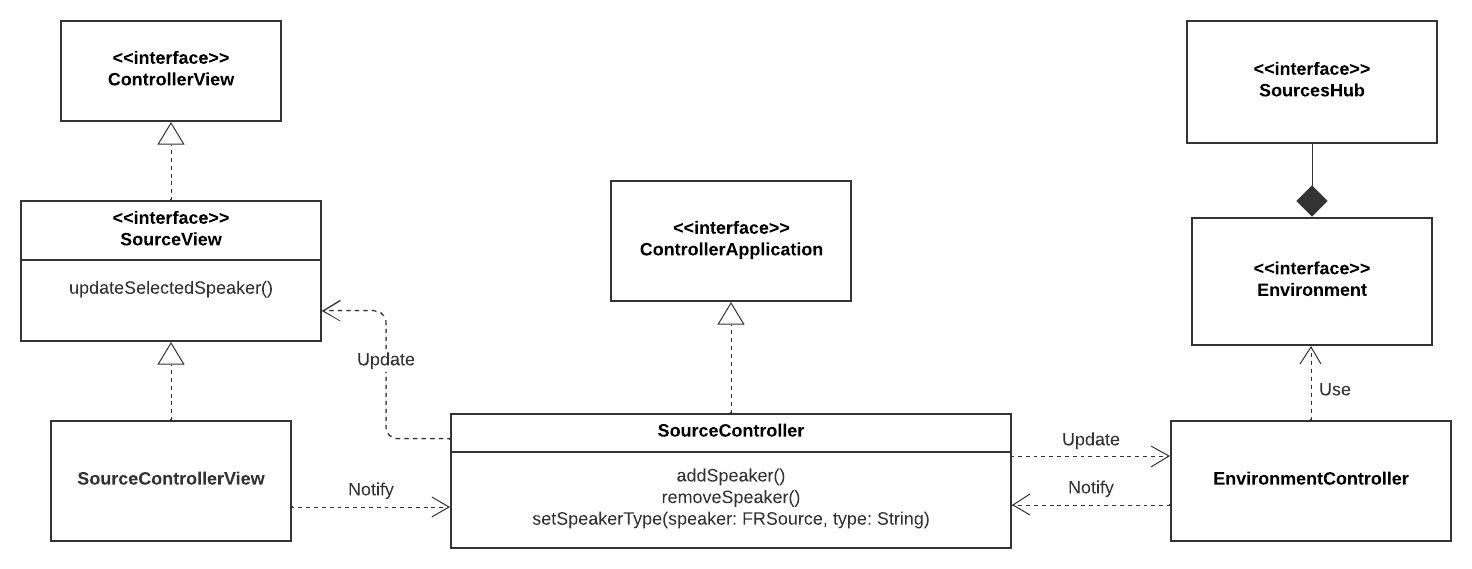
\includegraphics[width=\textwidth]{img/source/SourcesMVC.png}
\caption{Rappresentazione schematica MVC.}
\label{img:sourcesHub}
\end{figure}


\subsection*{Alex Presepi}
La progettazione e lo sviluppo da me affrontato riguarda principalmente due argomenti: Listener, e dei relativi plugin 
che ne estendono le funzionalita' visive e/o sonore.
\begin{figure}[H]
\centering{}
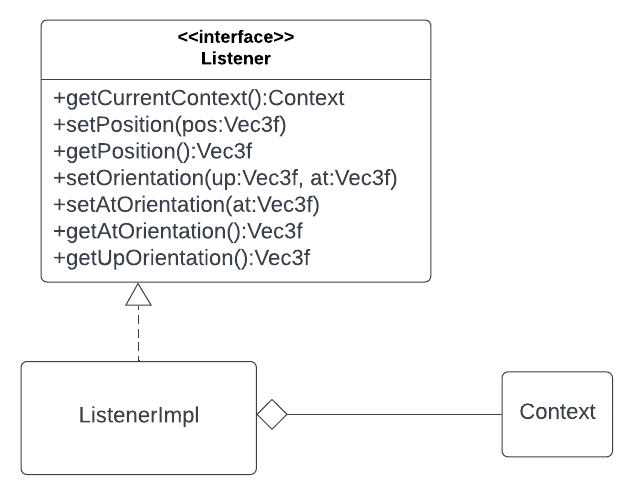
\includegraphics[width=\textwidth]{img/listener/Listener.png}
\caption{Rappresentazione UML dell'nterfaccia Listener e relativa implementazione.}
\label{img:Listener}
\end{figure}
%
Il Listener deve essere univoco in ogni contesto di eseguzione percio' per risolvere questo primo problema ho optato per creare una Simple Factory che permetesse di gestire l univocita per ogni contesto e mettesse a disposizione diverse modalita di creazione. Quando si richiama il metodo di creazione, 
passandogli il conteso di esecuzione, esso controllera se per quel contesto esiste gia un listener e ritorna o l istanza presente o ne crea una nuova. 
\begin{figure}[H]
\centering{}
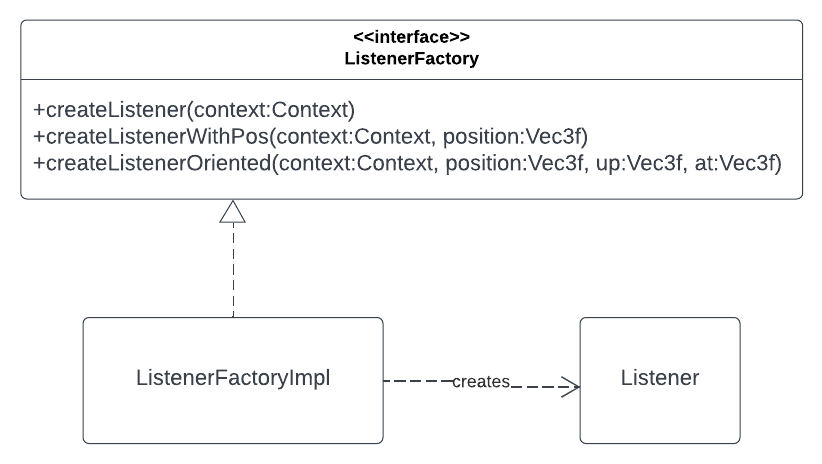
\includegraphics[width=\textwidth]{img/listener/ListenerFactory.png}
\caption{Rappresentazione della struttura Simple Factory.}
\label{img:Listener}
\end{figure}
%
Nello sviluppo dei Plugin volevo ottenere una struttura il piu modulare e estendibile possibile. Per prima cosa ho creato un interfaccia e una classe astratta che contenessero le operazioni di base. Inoltre ho usato un Tamplate method interno alla classe atratta (protected) per gestire il salvataggio e il ricaricamento dei setting ogni volta che si abilita o disabilita un Plugin.
\begin{figure}[H]
\centering{}
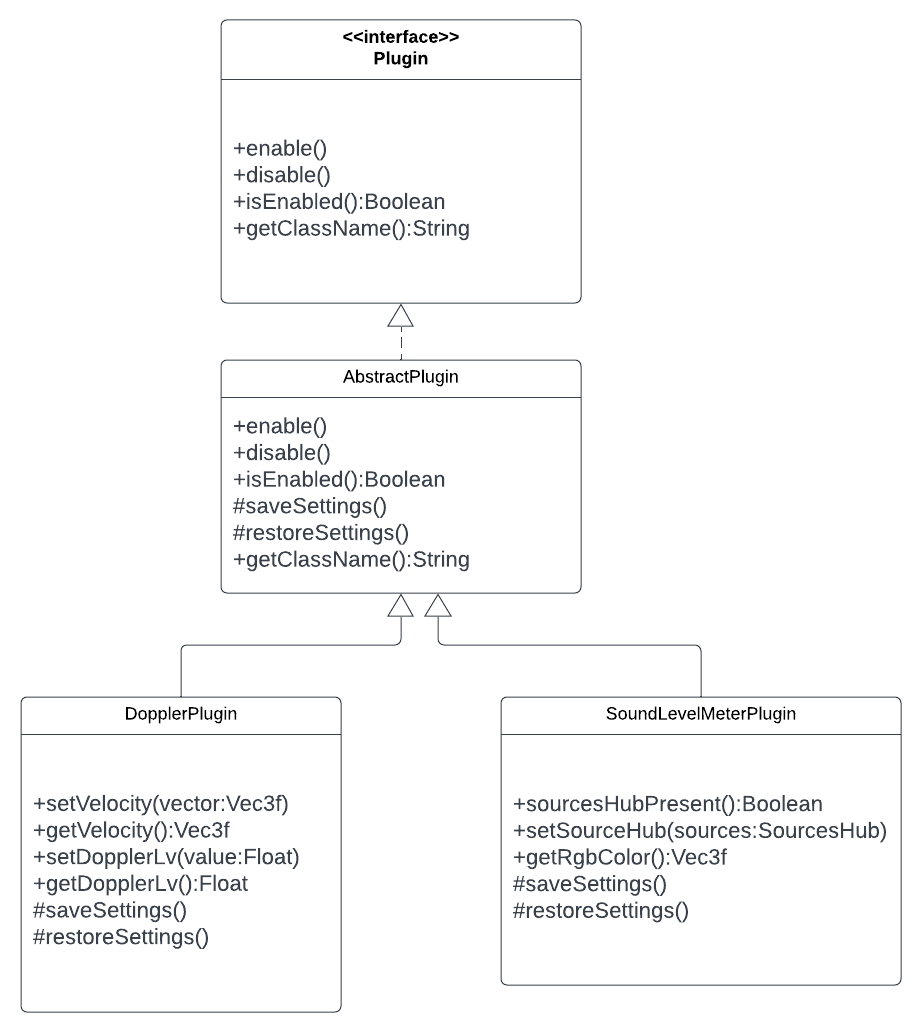
\includegraphics[width=\textwidth]{img/listener/Plugin.png}
\caption{Utilizzo di Tamplate Method in Abstract Plugin.}
\label{img:Listener}
\end{figure}
%
Per la gestione dei Plugin ho scelto di creare un classe che facesse da manager in modo da poter effetuare in modo semplice ed organizzato operazioni comuni su tutti i componenti gestiti. In ottica futura risultera' utille per poter getire piu listener, dove oguno avra' un proprio manager associato, o implementare e  gestire piu operazioni comuni tra Plugin.
\begin{figure}[H]
\centering{}
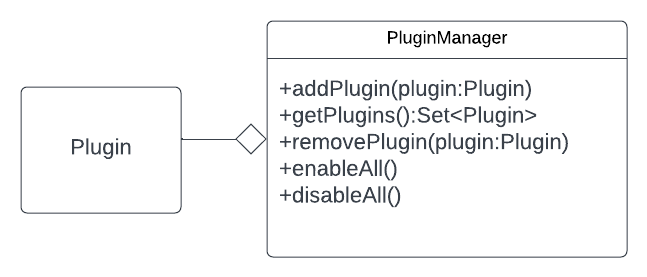
\includegraphics[width=\textwidth]{img/listener/PluginManager.png}
\caption{Schema UML della classe PluginManager.}
\label{img:Listener}
\end{figure}
%
La parte piu complessa nei Plugin e' stata:
\begin{itemize}
	\item la gestione del interfaccia utente.
	\item il caricamento di tutte le classi e risorse necessarie.
\end{itemize}
Per la comunicazione con la view ho creato un sotto pattern MVC. Cosi facendo lo sviluppo e l integrazione dei Plugin non influisce in alcun modo con
la struttura MVC dell' applicazione. Ogni plugin avra' quindi la propria parte di model, di controller, e di view (controller e FXML), come nel MVC generale. Inoltre e' presente un collegamento tra il controllerView del Plugin e il ListenerControllerView per aggiornare la view del applicazione, scelta dovuta dalla tecnologia grafica in uso. Infine ho reso possibile accedere, ai ControllerApplication (MVC generale), per dare la possibilita' di ottenere informazioni sullo stato del applicazione, mediante la composizione con il MainController.
\begin{figure}[H]
\centering{}
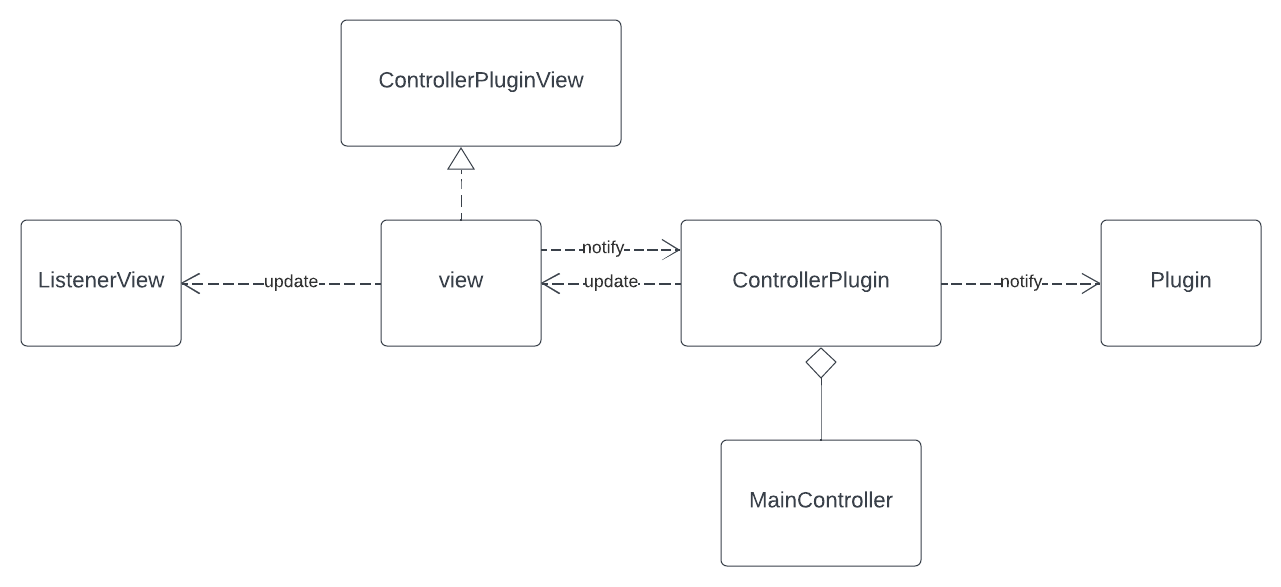
\includegraphics[width=\textwidth]{img/listener/PluginMVC.png}
\caption{Utilizzo pattern MVC nei Plugin.}
\label{img:Listener}
\end{figure}
%
Per il secondo problema mi sono avvalso del utilizzo delle Reflection. Questa decisione e' nata dal trovare una soluzione alla creazione di istanze di classi specifiche che in fase di compilazione non conosco. L utilizzo di esse aumenta l estendibilita' in quato l integrazione di plugin futuri e' resa possibile senza intaccare il codice del Applicazione. Il ListenerController crea via Reflection il ControllerPlugin desiderato e sara' esso a istanziare il model e la view relarive a quel determinato Plugin. TODO AGGIUNGERE SPIEGAZIONI 
\begin{figure}[H]
\centering{}
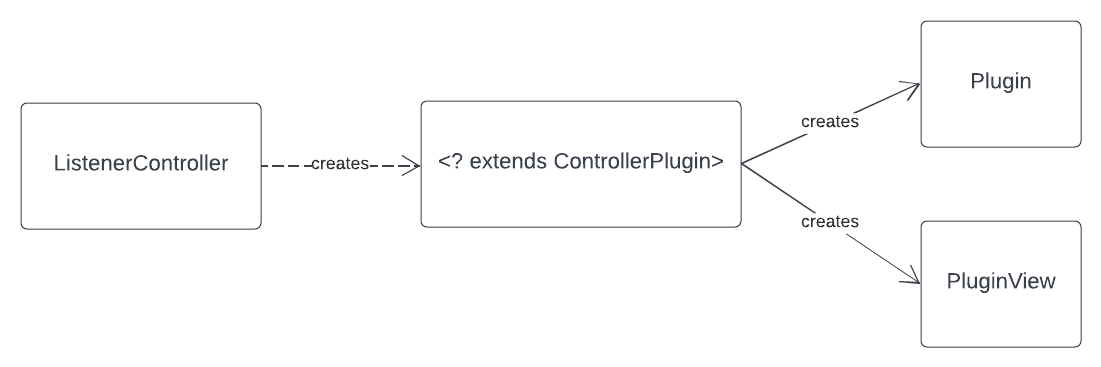
\includegraphics[width=\textwidth]{img/listener/PluginCreates.png}
\caption{Shema creazione Plugin.}
\label{img:Listener}
\end{figure}



\subsection*{Simone Lugaresi}
Due sono gli argomenti principali da me gestiti:
\begin{itemize}
	\item Space, che serve a delimitare uno spazio 2D di lavoro nel quale si potranno muovere Source e Listener.
	\item Environment, che è il contenitore di tutti gli elementi, sourceHub, Listener, space.
	\item AudioManager
\end{itemize}

\begin{figure}[H]
\centering{}
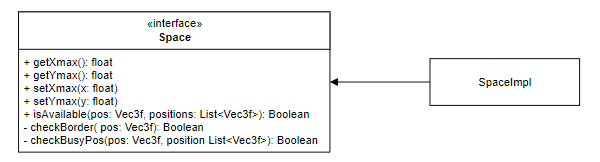
\includegraphics[width=\textwidth]{img/space/Space.png}
\caption{Rappresentazione UML dell'nterfaccia Space e la sua implementazione}
\label{img:space}
\end{figure}
Space si pone l'obbiettivo di risolvere il problema di delimitare uno spazio in cui poter utilizzare gli elementi, in questa implementazione viene utilizzato principalemte per fissare le dimensioni massime a Space che vengono costruiti nella factory di Environment, dato che la maggior parte dei controlli sulle posizioni vengono gestiti dalla View, rimane però la possibilita di controllare le posizioni degli spostamenti nell'ipotesi di un'interfaccia da console.
%
\begin{figure}[H]
\centering{}
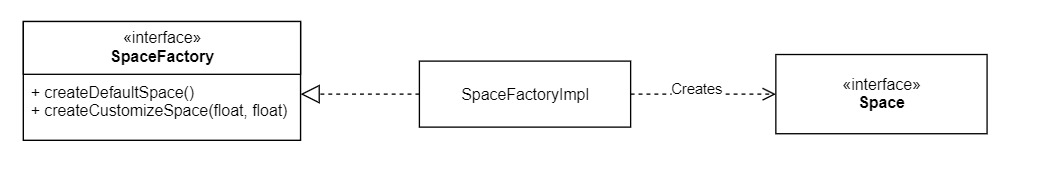
\includegraphics[width=\textwidth]{img/space/SpaceFactory.png}
\caption{Rappresentazione UML della Factory per Space}
\label{img:spacefactory}
\end{figure}
Per agevolare la creazione di Space, sia da utilizzare nei preset degli Environment sia per i Test, da la possibilità di scelta su due tipi di creazione di space, uno con dimensioni di default e uno con dei paramentri.
%
\begin{figure}[H]
\centering{}
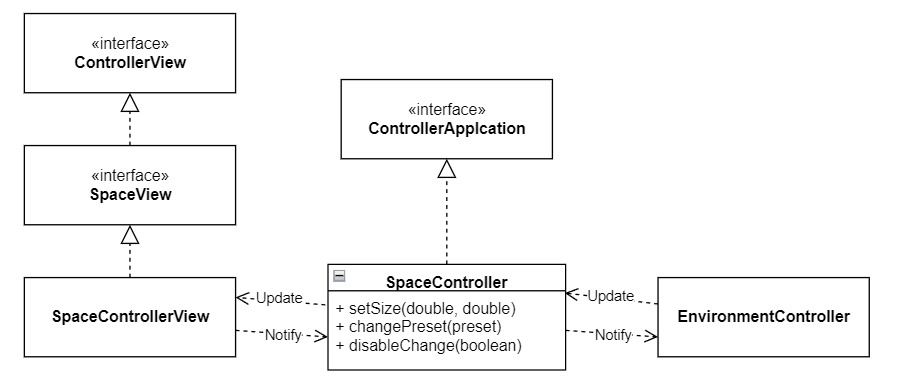
\includegraphics[width=\textwidth]{img/space/SpaceMVC.png}
\caption{Rappresentazione UML della gestione del MVC con space}
\label{img:spacemvc}
\end{figure}
La parte di MVC che riguarda space è molto semplice, nella sezione di SpaceView c'è  la possibilita di cambiare il tipo di environment tramite dei preset, e in più si agisce direttamente sulle dimensioni fisiche virtuali dello spazio in cui ono posizionati listener, e sources. Il tutto comunica con SpaceController che aggiorna o viene aggiornato a seconda delle circostanze da EnvironmentCotroller.
%
\begin{figure}[H]
\centering{}
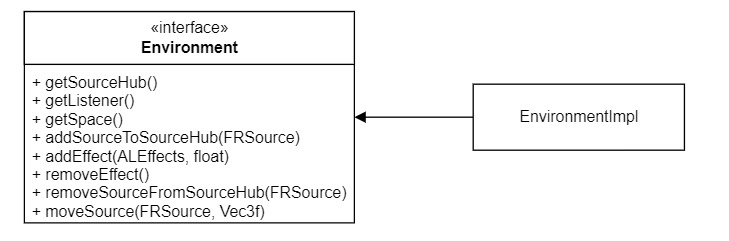
\includegraphics[width=\textwidth]{img/environment/Environment.png}
\caption{Rappresentazione UML della parte di Environment}
\label{img:environment}
\end{figure}
Per un miglior approccio agli elementi del programma quali listener, source, effects, Environment serve per raggruppare tutti gli elementi in un solo ambiente, in modo da poterlo rendere unico e riutilizzabile, anche in un ottica di un futuro aggiornamento nel quale si possono tenere aperti piu Environemnt e lavorare in contemporanea con essi.
Ho successivamente implementato la factory per poter creare Environment di default come Mono e Stereo, ma anche piu articolati come cinema e homeHIFI, in una sola riga.
%
\begin{figure}[H]
\centering{}
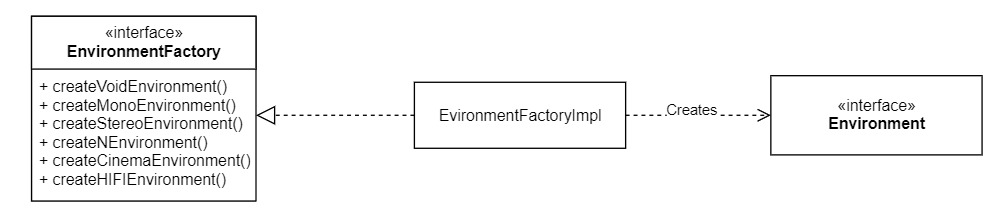
\includegraphics[width=\textwidth]{img/environment/EnvironmentFactory.png}
\caption{Rappresentazione UML della factory di Environment}
\label{img:environmentfactory}
\end{figure}

%
\begin{figure}[H]
\centering{}
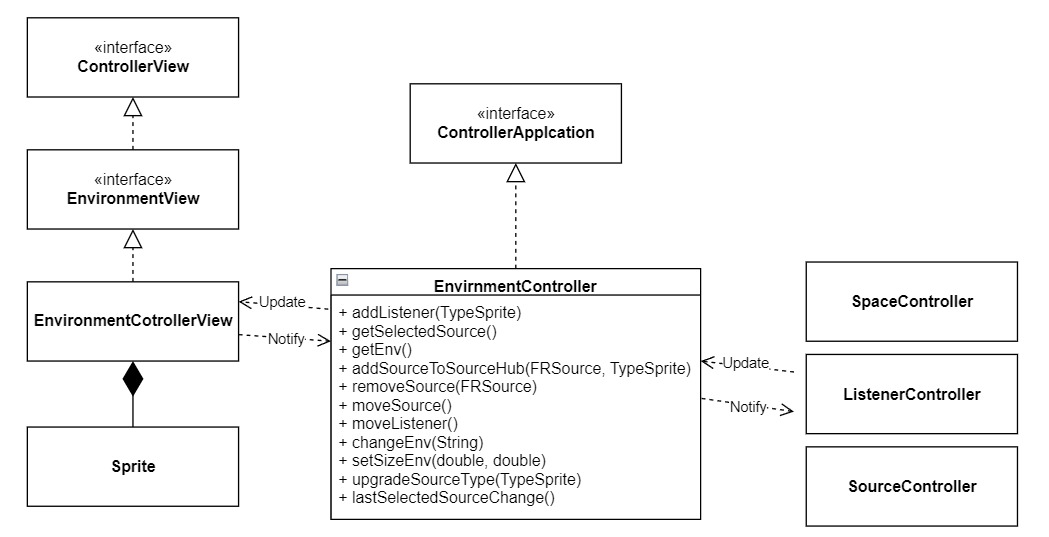
\includegraphics[width=\textwidth]{img/environment/EnvironmentMVC.png}
\caption{Rappresentazione UML della gestione del MVC con Environment}
\label{img:environmentmvc}
\end{figure}
La parte MVC di environemnt è formata da EnvironmentView che è ciò che comunica con EnvironmentController di envetuali cambiamenti avvenuti nella view, i quali possono essere solamente di un genere, ossia lo spostamente di un elemento nello space, di conseguenza EnvironmentController viene aggiornato, e aggiorna eventuali cambiamenti sui controller piu specifici come SourceController, ListenerController, SpaceController, ma anche EnvironmentView chen ha bisogno di essere aggiornata qualora ci siano aggiunte o rimozioni o cambiamenti di alcuni elementi come possono essere le source.
%
\begin{figure}[H]
\centering{}
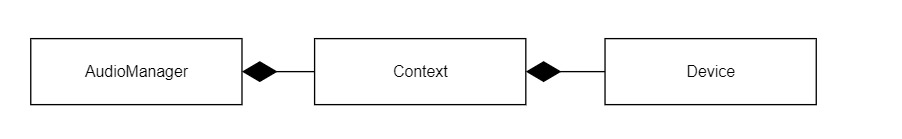
\includegraphics[width=\textwidth]{img/environment/AudioManager.png}
\caption{Rappresentazione UML dello schema semplice di AudioManager}
\label{img:audiomanager}
\end{figure}
Si tratta dell'implementazione di tre classi semplici, che pero sono necessarie per una corretta comunicazione con la libreria e le nostre classi. Servono per creare il contesto nel quale le source dovranno riprodurre i suoni e il listener dovra riceverli.
%

\chapter{Sviluppo}
\section{Testing automatizzato}
La suite utilizzata per i test automatizzati è JUnit. Durante il processo di implementazione siamo stati accompagnati dai test effettuati tramite le actions di GitHub, che ne verificavano l'assenza di errori sui principali sistemi operativi (Windows, MacOSX, Ubuntu).
\\In particolare, si è deciso di sottoporre a test automatizzato i seguenti componenti:
\begin{itemize}
	\item Buffer: test di caricamento sia attraverso file system sia da classpath, oltre al test del corretto funzionamento del caching.
	\item Filter: test di applicazione dei tre tipi di filtri su delle sorgenti.
	\item Space: test di una corretta esecuzione dei metodi, e dei loro risultati con determinati input.
	\item Environment: test di corretta counicazione tra tutti gli elementi presenti dentro Environment, e i suoi metodi.
	\item Listener: 
	\item Source: 
	\item Plugin: 
\end{itemize}
Altre funzionalità richiedevano un test uditivo per verificarne la correttezza, che ci era difficile verificare in modo automatizzato.
%
\section{Metodologia di lavoro}
Una ingente parte di ricerca è stata svolta prima della creazione del progetto e dell'analisi, poichè avevamo la necessità di verificare la fattibilità del progetto che avevamo ideato e che ha comportato la valutazione di varie librerie con tutto quello che ne consegue, come test di prototipi e studio delle documentazioni. La scelta finale è ricaduta su OpenAL, cercando successivamente librerie Java che facessero da API ad essa, di cui abbiamo valutato JOAL e LWJGL, selezionando quest'ultima dopo un'analisi dei pro e contro di entrambe da cui abbiamo riscontrato incompatibilità critiche in JOAL.
\\Visto che nessuno dei componenti aveva esperienza pregressa nell'utilizzo di GitHub in progetti di questa entità, abbiamo optato per una gestione di base attraverso una semplice strategia "push e pull", lavorando spesso sullo stesso branch, salvo poche eccezioni, per evitare complicazioni e concentrarci sulla pura implementazione.
\\Il lavoro in comune è stato effettuato per definire le interfacce che servivano come punto di accesso tra le diverse parti, nei componenti "manager" (come MainController e MainControllerView) e nei vari package utility.
\subsection*{Niccolò Mussoni}
Buffer, BufferCache, view per l’importazione di un file WAV, Extensions (effetti + filtri), view per l’applicazione degli effetti su tutte le sorgenti attraverso un semplice equalizzatore
\subsection*{Alessandro Sciarrillo}
\subsection*{Alex Presepi}
\subsection*{Simone Lugaresi}
Environment, Space, view per la gestione degli elementi all'interno della canvas, view per la gestione degli spazio simulati.
\section{Note di sviluppo}
\subsection*{Niccolò Mussoni}
\begin{itemize}
	\item Lambda expressions
	\item Stream
	\item Optional
	\item JavaFX, per la GUI
	\item LWJGL, libreria audio su cui si basa l’intero progetto
	\item Spring Framework, per accedere a tutte le risorse all’interno di una cartella del classpath
	\item Per la conversione da WAV stereo a WAV mono mi sono affidato a del codice online, non avendo le competenze necessarie per manipolarlo, che ho poi adattato alla singola conversione di cui necessitavo: \url{http://www.java2s.com/example/java/javax.sound.sampled/converts-re-samples-and-mono-tofrom-stereo-audio-data.html}
\end{itemize}
\subsection*{Alessandro Sciarrillo}
\subsection*{Alex Presepi}
\subsection*{Simone Lugaresi}
\begin{itemize}
	\item Lambda expressions
	\item Stream
	\item Optional
	\item JavaFX, per la GUI, e la gestione degli sprite
	\item OpenAL, libreria audio su cui si basa l’intero progetto
\end{itemize}

\chapter{Commenti finali}
\section{Autovalutazione e lavori futuri}
\subsection*{Niccolò Mussoni}
\subsection*{Alessandro Sciarrillo}
\subsection*{Alex Presepi}
\subsection*{Simone Lugaresi}

\section{Difficoltà incontrate e commenti per i docenti OPZIONALE}

\appendix
\chapter{Guida utente}

\chapter{Esercitazioni di laboratorio}
\subsection*{Niccolò Mussoni}
\begin{itemize}
	\item Laboratorio 05: \url{https://virtuale.unibo.it/mod/forum/discuss.php?d=87881#p136373}
	\item Laboratorio 06: \url{https://virtuale.unibo.it/mod/forum/discuss.php?d=87880#p139071}
	\item Laboratorio 07: \url{https://virtuale.unibo.it/mod/forum/discuss.php?d=88829#p136368}
	\item Laboratorio 08: \url{https://virtuale.unibo.it/mod/forum/discuss.php?d=89272#p139072}
	\item Laboratorio 09: \url{https://virtuale.unibo.it/mod/forum/discuss.php?d=90125#p138604}
	\item Laboratorio 10: \url{https://virtuale.unibo.it/mod/forum/discuss.php?d=91128#p139736}
\end{itemize}

\subsection*{Alessandro Sciarrillo}
\subsection*{Alex Presepi}
\subsection*{Simone Lugaresi}
\begin{itemize}
	\item Laboratorio 05: \url{https://virtuale.unibo.it/mod/forum/discuss.php?d=87881#p136825}
	\item Laboratorio 06: \url{https://virtuale.unibo.it/mod/forum/discuss.php?d=87880#p136726}
	\item Laboratorio 07: \url{https://virtuale.unibo.it/mod/forum/discuss.php?d=88829#p136582}
	\item Laboratorio 09: \url{https://virtuale.unibo.it/mod/forum/discuss.php?d=90125#p138776}
	\item Laboratorio 10: \url{https://virtuale.unibo.it/mod/forum/discuss.php?d=91128#p140008}
\end{itemize}

\tableofcontents

\end{document}
